\documentclass[12pt]{revtex4}
\usepackage{ulem}
\usepackage{url}
\usepackage{epsfig}
\usepackage{graphicx,color}% Include figure files
%\usepackage{epstopdf}
\DeclareGraphicsRule{.tif}{png}{.png}{`convert #1 `basename #1 .tif`.png}
\usepackage[psamsfonts]{amssymb}
\usepackage{amsmath}
\usepackage{indentfirst}
%\usepackage{cite}

\newcommand{\be}{\begin{equation}}
\newcommand{\ee}{\end{equation}}
\newcommand{\ba}{\begin{eqnarray}}
\newcommand{\ea}{\end{eqnarray}}

\begin{document}
%\title{Patterns of Human Learning in Complex Systems}
\title{Do modern humans solve problems with \\ algorithms used by hunter-gatherers in search for food?}

\author{Thomas Maillart}
\email{thomas.maillart@unige.ch}
\affiliation{University of Geneva, Geneva, Switzerland}

\author{Johannes Castner}
\email{jcastner@ebay.com}
\affiliation{Ebay Research,
San Francisco, USA}




\date{\today}


\begin{abstract}
%\vspace{1cm}
Recent research \cite{baronchelli2013levy} has suggested that cognitive mental search patterns \cite{rhodes2007human,radicchi2012rationality,radicchi2012evolution} may be inherited from typical foraging and mobility patterns of animals \cite{viswanathan1996levy,ramos2004levy,reynolds2007displaced} and humans \cite{gonzalez2008understanding,song2010mode\
lling,rhee2011levy}. In particular, patterns suggest that cognitive processes in abstract spaces are similar to food search algorithms of hunter-gatherers, modeled as L\'evy flights \cite{brown2007levy,raichlen2014evidence}. Here, we study the mental search trajectories of
individuals who have been asked to reverse engineer the conditional probabilities of 3-variable and 4-variable stochastic processes, as Bayesian
networks (48 participants per treatment) \cite{steyvers2003inferring,pearl2009causality}. We find an important contrast with the random trajectories predicted by L\'evy flight and random walk models, optimized for search of sparse targets %\cite{viswanathan1999optimizing,edwards2007revisiting,song2010modelling\
,viswanathan2011physics}.  
Human mental search exhibits temporal and spatial regularity, characterized by a time dependent distance between two consecutive solutions proposed by each individual.  Additionally, we find an unexpected tendency to return to previously tested solutions.  Both, contribute to a sub-optimal exploration of the
problem space, which in turn slows the speed of approaching the target solution.  Our results
suggest that inherent cognitive limitations hinder efficient exploration of complex abstract spaces.  These limitations appear to be hard-wired in our brain, and may stem from previously evolutionary fit hunting strategies that are inefficient for solving hard problems in modern environments. 

\end{abstract}

\maketitle

\section{Introduction}
In scientific research \cite{}, software engineering and cybersecurity \cite{}, politics \cite{}, and daily life \cite{}, individuals face problems that involve many interdependent variables and thus large problem spaces, although only sparse -- or unique -- solutions exist \cite{}. These problems are known to be hard to humans, and have been studied by cognitive scientists \cite{Neurath's boat}. In cognitive science, reverse-engineering a Bayesian Network, which involves complicated interdependencies, has become a typical way to probe cognitive capabilities \cite{}. Because variables are dependent, landscapes are not smooth and solutions cannot be reached by simple local search/optimisation strategies {\bf (could we illustrate this point in a way or another with a figure?)}. 

Here, we investigate the fine-grained cognitive mechanisms of complicated problem resolution, which involves 2 treatments {\bf for} the resolution of 3-node and 4-node Bayesian networks over one trial of XX minutes, with a warm-up period of YY. Reverse-engineering these Bayesian networks involve evaluating respectively 8 and 16 conditional probabilities (varying from $0$ to $1$). Any change to any of these probabilities is registered with a resolution of one second [see Supplementary Information (SI) \ref{SI_experiment}]. On average, participants perform poorly in both treatments (see Figure \ref{fig:1}A), and improvement of the proposed models over time follows an extremely slow decay [with Jensen-Shannon Distance $D_{jsd}(t) \sim t^{\nu}$ with $ \nu \approx -0.15(1)$]. 

\begin{figure}[h!]
\begin{center}
\includegraphics[width=17cm]{figures/figure1.eps}
\caption{\footnotesize{{\bf A.} Average Euclidian Distance $\langle D \rangle$ decays as function of time as $\sim t^{\nu}$ with $ \nu \approx -0.15(1)$ indicating a very slow convergence to the true model {\bf [indicate $t_0$s and what their values may mean]}. {\bf B.} Probability density function of displacement $pdf(\Delta r) = \Delta r^{-\alpha -1}$ with $\alpha = 0.40(5)$ with a cut-off limited by the largest possible displacement, which is $\sqrt{k}$ with $k$ the number of conditional probabilities to evaluate. {\bf C.}  Probability density function of waiting time $\Delta t$ $pdf(\Delta t) = \Delta t^{-\beta -1}$ with 2 regimes : $\beta_{\Delta t < 125} = 0.38(4)$ and $\beta_{\Delta t > 125} = 1.59(5)$. Distributions of $\Delta r$ and $\Delta t$ are equivalent for the simple and complex treatments.}}
\label{fig:1}
\end{center}
\end{figure}

Humans -- like many other animals \cite{} -- use efficient strategies to search for food over large areas \cite{rhodes2007human}. These L\'evy walks strategies alternate many small local displacements and few long range displacement. Namely, the distribution of displacements obeys a power law: 

\begin{equation}
\label{displacements}
pdf(\Delta r) = \Delta r^{-\alpha -1}.
\end{equation}

We find that displacements between proposed models (on average over all participants) follow a similar power law distribution with $\alpha = 0.40(5)$ (see Figure \ref{fig:1}B). In addition, the distribution of waiting times $\Delta t$ between two iterations of model propositions, also follows a power law: 

\begin{equation}
\label{wtimes}
pdf(\Delta t) = \Delta t^{-\beta -1},
\end{equation}

with 2 regimes : $\beta_{\Delta t < 125} = 0.38(4)$ and $\beta_{\Delta t > 125} = 1.59(5)$. Distributions of $\Delta r$ and $\Delta t$ are equivalent for the simple and complex treatments. Together, equations \ref{displacements} and \ref{wtimes} define a Continuous Time Random Walk (CTRW) \cite{}, which is another flavour of food search for {\bf XXXanimals} in ecological systems \cite{book_ecological_systems}. The observed displacement exponent is significantly smaller, compared to optimal L\'evy walks of food search in ecosystems, typically found close to  $\alpha = 1$ \cite{} and mathematically optimal for search of sparse solutions in wide areas, provided that search is a memoryless process \cite{viswanathan1999optimizing, edwards2007revisiting,song2010modelling,viswanathan2011physics}. \\

\subsection{Memory in L\'evy Walks/Flights}

However, humans exhibit repeated behaviours, which imply memory. For instance, evidence from online auctions \cite{radicchi2012rationality}  suggests that optimal search strategy ($\alpha = 2 $) can be reached by humans when considering evolutionary forces \cite{radicchi2012evolution}. Sedentary human mobility (e.g., in cities) also exhibits repeated travel behaviours, such as between home and work places, with short displacements around few areas of particular interests, and with punctual travels beyond the borders of the city, e.g., to another city or country \cite{brockmann2006scaling,gonzalez2008understanding,song2010modelling}. Using mobile phone traces, Song et al.  have proposed a modified version of L\'evy flights, by incorporating a form of preferential attachment, which predicts that most visited places tend get even more visits \footnote{The model proposed by Song et al. \cite{song2010modelling} is however a challenge to common sense logic: Most visited places (i.e., home and workplace) are visited at a stable rate, roughly following circadian periods.}. Yet, on the contrary to early models \cite{viswanathan1999optimizing, edwards2007revisiting,song2010modelling,viswanathan2011physics}, proposed explanations by Radicchi et al. \cite{radicchi2012evolution} and Song et al. \cite{song2010modelling} incorporate memory, either through evolutionary forces to optimise online auction strategies (through {\it try and fails}), or human memory driving routine repeated visits of same places \cite{gonzalez2008understanding,song2010modelling}, because they bring renewal resources (mainly financial resources are derived from staying at work, while home may bring e.g., a roof for the night, rest and intrinsic rewards). {\bf Although we have not found documented evidence of memory for animals and nomad humans (such as e.g., hunter gatherers), they may similarly perform L\'evy flights with memory, returning to previously visited food spots, which have replenished between two visits [$\rightarrow$ is there a chance to find evidence for this, even if it's qualitative? I am really surprised this has not been documented yet.]}.\\

%\ref{fig:3}A ???


\subsection{An experiment to probe cognitive mechanisms involved for solving hard problems}

Hard problems {\bf [provide a strict definition of hard problems above, as much as possible, or refine terminology]} have a unique best solution, which can be approached. yet getting close to this solution is hard, because many interdependent variables are involved. 

Individuals tackling hard problems face a tension between testing and updating their beliefs from information stored in their memory (i.e., {\it exploitation} or {\it recombination of information}), and taking action to {\it explore} and update their belief from not previously available {\it exogenous} information. Taking such action would equivalent to the exploration of unknown territories by pioneers in the physical world. The former {\it exploitation} approach may bring improvement toward the solution, however limited to a {\bf (linear?) combination} of previously tried solutions. The latter approach is a {\bf more} high-risk high-return strategy, but whether it brings improvement towards the solution or not, it matters little, as this strategy primarily expands the {\bf convex hull of the explored portion of the solution space [not sure if we can say it this way]}. Once a new portion of the solution space has been explored, the attempted proposed model is then stored into memory and may be recombined, later on, with other proposed models. \\
\begin{figure}[h!]
\begin{center}
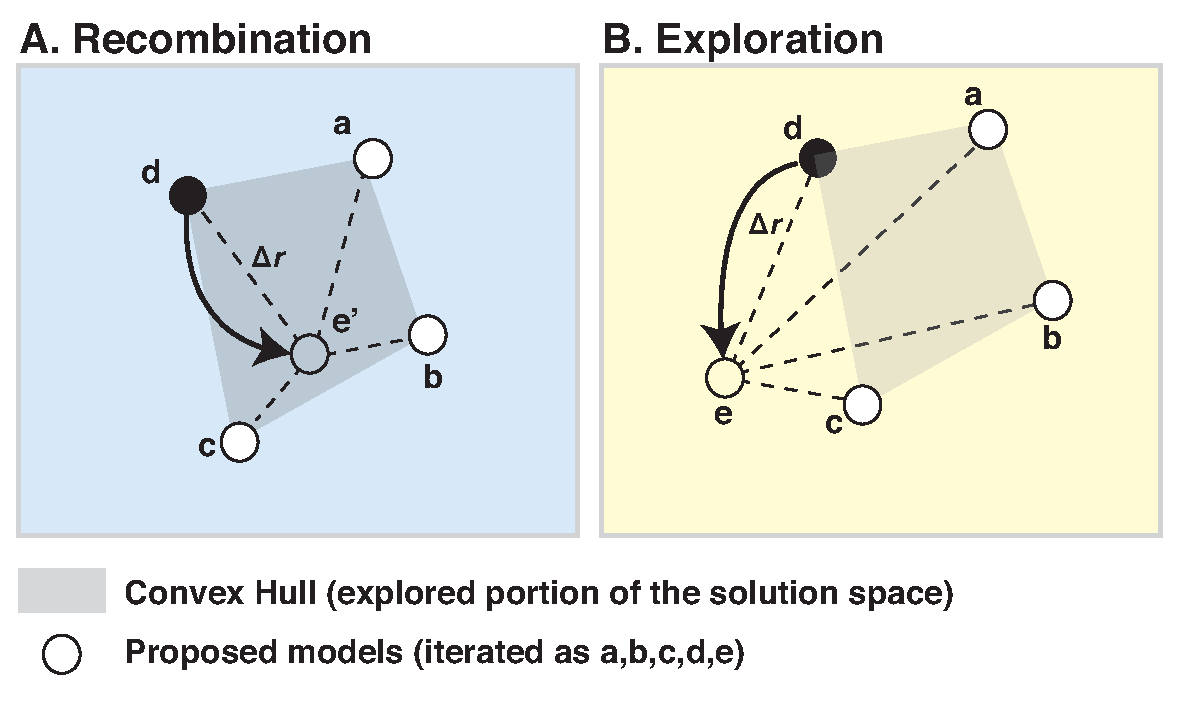
\includegraphics[width=12cm]{figures/figure2.eps}
\caption{\footnotesize{Simplified diagram of exploration and recombination on a plane: {\bf A. Recombination:} iteration {\bf e'} does not incorporate new information. It is a {\bf (linear?)} combination of all previous proposed solutions (i.e., $\{a,b,c,d\}$).  {\bf B. Exploration:} the average distance between iteration {\bf e} and all previous iterations is larger than half of the maximum distance between any previous proposed solutions. Exploration is not memoryless: {\bf e} is closer to {\bf c} and {\bf d} than {\bf a} and {\bf b}. }}
\label{fig:2}
\end{center}
\end{figure}

There is a dearth of knowledge on how the exploration out of the convex hull brings new information, which is then recombined with previously acquired knowledge, stored in memory (see Figure \ref{fig:2}A). Exploration is not memoryless and still occurs by leveraging memory (see Figure \ref{fig:2}B). While exploration entails a pure luck component (beyond the previously explored convex hull), recombination could be optimised to find the best possible recombination, which corresponds to the optimal proposed solution (i.e., as close as possible from the true solution) within the currently explored convex hull.\\

The experiment conducted at Columbia University Social Science laboratory with 96 participants asked to reverse engineer a Bayesian Network with its conditional probabilities and dependencies between nodes show the very fine grained mechanisms of how people struggle balancing recombination of information stored in memory and exploration beyond the currently known convex hull as a subset of the solution space. Our results suggest that displacement $0.1 < \Delta r < 0.2 $ is particularly beneficial for making progress toward the correct solution. We also find that large displacements orders of magnitude more ``brain processing" time compared to small displacements {\bf [how can we make sure that this is truly brain processing time and not an artefact from the web interface?]}. Displacement $0.1 < \Delta r < 0.2 $ is precisely at the inflexion point before waiting times get punishingly long. Yet it remains unclear if some participants manage to consistently use this {\bf ``best strategy"} or if performance is mainly a matter of luck.


This article is organized as follows. We first report on the experimental results, in particular deviations from a memoryless L\'evy Walks/Flights, such as peculiar returns to previously visited solutions, {\bf anomalous mean square displacement following return and recombination [more work is needed here]}, explorations beyond the convex hull, as well as waiting-time and long-memory processes. We then show memory, exploration and recombination influence performance. {\bf Building on theoretical consideration in conjunction with observed stylized facts, we test a model of mechanics of cognition when people tackle hard problems [remains to be done. It may incorporate some Hawkes Processes, but not 100\% sure yet]}. 



\clearpage

%The cognitive  as well as the evolutionary \cite{radicchi2012evolution} underpinnings of L\'evy walks by humans has been questioned and investigated. The ramifications of L\'evy walks in the mind with foraging / mobility patterns in the physical space: here we question if 
%our mind has been shaped by evolutionary pressure and humans resort to similar strategies. Recent research on online bids \cite{radicchi2012rationality} found similar L\'evy walk patterns even though they appear sup-optimal and even slightly irrational, hence suggesting that L\'evy walks are somehow hard coded in our mind  \cite{radicchi2012evolution}, as humans resort to search strategies, which are no longer fit in the world of information and reasoning with abstract problems, which resolution brings its own incentives and resource rewards in the form of money, recognition, reputation, and pleasure \cite{rewards_modern_societies}.\\

%Here, considering humans facing a hard problem -- typically a unique solution in a complicated problem space -- mental search patterns may be inherited from similar L\'evy walks/flights foraging and mobility patterns �\cite{rhodes2007human,radicchi2012rationality,radicchi2012evolution}.\\

%However, these findings were based on specific cases, involving a specific type of auctions \cite{baronchelli2013levy}. It is also considered that the strategy used is L\'evy walks/flights because it is optimal. However, only truly random L\'evy walks/flights are optimal. True randomness is equivalent to a memoryless process, which would allow exploring the solution space with no consideration of previous knowledge. (a evolutionary theory framework is used to rationalise their findings).\\

%Searching for (or tending/optimizing to) a unique solution involves try and fail, and progressive learning. One may think of an evolutionary process (e.g., ``Animals explore the environment mainly for searching food resources, and it is therefore plausible to ascribe the optimality of their search strategies to a selective evolutionary process."  \cite{radicchi2012evolution}), a Markov process \cite{}, or a process with long range memory, in which candidate solutions explored in the past are reused, and recombined with more recent explored solutions. Finally, some new solutions are truly explored out of the currently explored solution envelop.\\
 
% \subsection{Experiment}
%In our experiment, participants were asked to reverse engineer a Bayesian network. They were given 40 minutes, and all changes made were recorded at a 1 second resolution. Participants trying to reverse the best solution face a though problem: The {\it simple} Bayesian network has 3 nodes, and is defined by a 8-parameters vector $\mathbf{s}$ with $0 \leqslant s_k  \leqslant 1$ for $k = \{1,...,8\}$ (resp. $k = \{1,..., 16\}$ for the 4 node {\it complex} Bayesian network). 
 
 
%\subsection{L\'evy Flight / CTRW}
%We first find that the search process follows a L\'evy flight process with waiting times between moves are random variables, which can be accounted together as a continuous time random walk. Both the distributions of displacement (Figure \ref{fig:pdfs}A ) and waiting times (Figure \ref{fig:pdfs}B ) exhibit power law distributions  (Probability density function of displacement $pdf(\Delta r) = \Delta r^{-\alpha -1}$ with $\alpha = 0.40(5)$. {\bf B.} Probability density function of waiting time $\Delta t$ $pdf(\Delta t) = \Delta t^{-\beta -1}$ with 2 regimes : $\beta_{\Delta t < 125} = 0.38(4)$ and $\beta_{\Delta t > 125} = 1.59(5)$. Distributions of $\Delta r$ and $\Delta t$ are equivalent for the simple and complex treatments.){\bf Problem :} Such CTRW process should normally follow ballistic diffusion characterized by mean square displacement (MSD) and diffusion $\sim t^{\mu}$ with  $\mu_{Levy} = 1$ or super-diffusion $\mu_{CTRW} = \beta$ \cite{21,23}). Here, however, mean square displacement (MSD) decays as $\sim t^{\mu}$ with $\mu_{simple} =-0.23(2)$ and $\mu_{complex} =- 0.26(1)$ showing a slow convergence. 

 
 %Here, we document how such frustrating and somewhat irrational situations may stem from evolutionary homology \cite{evolutionary_homology}, that is mental search properties may share conserved neural substrates with similar neuro-molecular processes guiding spatial search in animals and modulating the control of human attention \cite{hills2006animal}. We show that search strategies inherited from food \cite{food_foraging} and resource \cite{resource_foraging} foraging lead to a form of ``hard-wired bounded rationality" when tackling hard problems.\\

%This behavior is at odds with L\'evy walks food search strategies 
%\cite{iswanathan2011physics} used by number of animals 
%\cite{viswanathan1996levy,reynolds2007displaced,edwards2007revisiting,ramos2004levy} and hunter gatherers 
%\cite{brown2007levy}. L\'evy walks which displacement obeys a power law distribution 
%$P(R > \Delta r) \sim \Delta r^{\alpha}$ with $ 0 < \alpha \leqslant 2 $ are known maximize 
%displacement through a super-diffusive process, while minimizing the probability to return to an 
%already visited site (on the contrary to Brownian motion \cite{humphries2010environmental,mendez2013stochastic}). In 
%particular, the food search process in nature has also been found to be optimal $\alpha \approx 1$ 
%\cite{viswanathan1999optimizing}, in the case of Hadza hunter-gatherers in Tanzania 
%\cite{raichlen2014evidence}, and for the dissemination of mussels \cite{de2011levy}. In the latter 
%case, the optimal search process stems from the cooperative organization of mussels, and how 
%this cooperation shapes the environment \cite{de2011levy}. Human mobility traced by banknote circulation \cite{brockmann2006scaling} or mobile phone tracking \cite{song2010modelling,rhee2011levy} also exhibits highly regular L\'evy walk patterns \cite{gonzalez2008understanding}.

%There is suggestive evidence that some cognitive mechanisms, such as information/memory retrieval follows a L\'evy walk \cite{hills2012optimal} with some limited analogy with optimal foraging \cite{rhodes2007human} {\bf (in \cite{rhodes2007human}, it's unclear why the waiting times should be optimal with $\mu \rightarrow 1$. The optimality is in space, optimality is less clear in time)}. {\bf (random walks \cite{abbott2015random})}

%For some time now, cognitive scientists have posed that modeling people's beliefs about causation in the material world provides an effective explanatory framework for how we process information and learn from these observations \cite{Griffiths2008}.  Probabilistic causes and effects, in other words, make up an important construct we seem to make use of when we seek to understand our world.  Bayes Nets are well-defined mathematical objects corresponding to an intuitive representation of causal beliefs.  They are easy to manipulate, do inference with and use as a means to compare different beliefs.  The kinds of Bayes Nets that have been allowed for in experimental settings up to this point, however, have been extremely simplistic and there has been an unanswered call for learning experiments with increased complexity (Griffiths?).  Our work is to our knowledge the first answer to this call.

%From financial stability to the stability of democracies, beliefs play a central role in our explanation of many phenomena. In the social sciences, these beliefs are often conceptualized as probabilistic assessments over states of the world.  However, they are derived from coherent belief systems people hold in their minds regarding how the world works as supported by recent work in cognitive science \cite{lombrozo2006structure, anderson1990cognitive}.  How do humans learn in simple and in complex systems?  How efficiently do they explore the space of possible beliefs and how closely is the direction of exploration tied to experience?  Bayesian approaches of learning would not be feasible for learning in realistically complex systems, given recall constraints and they are not defined in cases where initial beliefs are such that they put zero weight on some possible outcomes.

%Our work presents new experimental results on the rate at which people learn in more or less complex environments. We find that learning rates are much slower than they would be if learners were Bayesians, as had been proposed in older economic theories \cite{Boyer84, Prescott72, Rothschild74, McLennan84, Mirman84, Easley89, Kiefer89}. We also find that the learning rate is slightly higher when people build models of systems that are less complex and that even if the rates were identical accross levels of complexity, accuracy is always higher when the system is structurally simpler because initial models are closer aligned with reality.

%When searching for solutions to outstanding problems, in this case the formation of coherant belief structures that explain experience, humans must come up with innovative solutions.  We show that their strategies look a lot like a class of random search processes in which complete random guessing is strategically combined with the consolidation of past and current experience. We show how people shape their beliefs, starting with complete guesswork through a process that can be accurately modeled as a L'evy random search process, which involves both synthesis of current knowledge (mental exploitation) and out-of-the box mental exploration (see Figure \ref{fig:schematic}). Such random search processes are ubiquitous across the life sciences, in cognitive science, computer science  and artificial intelligence. We then measure how this process leads to convergence, albeit slow, to the correct stochastic solution.

%As can be seen in Figure \ref{fig:decay}, the distance between a person's evolving belief system about some physical system and the long-run absorbing distribution, which we interpret as a performance score, decays with time in a very specific way:
%
%\begin{equation}
%\label{ }
%d(belief_{i, t}, absorbing distribution) = \alpha*t^{-\beta_i}
%\end{equation}
%
%The functional form of human learning in the context of our experiment, then, is the same as for the Bayesian learner, but the decay rate, $\beta$, of a human learner is much smaller than that of a Bayesian.

%\section{Background}
In general, when sentient beings (humans or other animals) search and find solutions to their problems, this brings rewards.  At times, the solution is its own reward \cite{hedonism}, but more often the reward is survival \cite{smith_optimization_1978}, which implies finding resources directly (foraging) or indirectly (through monetary means). To strive, food search shall be economic, i.e., the search cost shall not be larger than the energetic intake \cite{pyke_optimal_1984} and optimization shall occur through either ``time minimization'' (time spent feeding is traded off for time spent on other activities) or ``energy maximization'' (fixed time in which to feed during which the animal aims to maximize its energy gain) \cite{schoener_theory_1971}.\\

The evolution of foraging behavior is subject to functional (e.g., morphologies and physical properties \cite{pyke_optimal_1984}) and environmental constraints (e.g., distribution and accessibility of food patches on complex environmental landscapes \cite{}). The capacity to sense, store and process foraging information is critical \cite{kamil_learning_1982}. Animals may obtain information through either direct experience, observation of others \cite{weigl_observational_1980}, or through basic or advanced collective intelligence mechanisms \cite{}. Foraging strategies are also assumed to evolve more rapidly than the rate at which relevant conditions change \cite{pyke_optimal_1984}. In that sense, animals are expected to adapt and optimize their foraging behaviors \cite{pyke_optimal_1977}.\\

%{\it If the animal is alone in a uniform environment, no difficulty arises.
%But if we allow for competition and for a changing environment, several
%choices of optimization procedure are possible. For example, three 
%possibilities arise if we allow just for competition:} $\rightarrow$ capacity 
%to anticipate, build relevant scenarios </Maynard1984> 

Foraging in natural environments often entails finding sparsely distributed food sites. \cite{levandowsky_swimming_1988} have suggested that microorganisms may search for sites following a Levy flight process, defined as 

\be
eq~Levyflight
\ee 

A Levy distribution is advantageous  when target sites are sparsely and randomly distributed, because the probability of returning to a previously visited site is smaller than for a Gaussian distribution. The Levy flight may also help overcome the problem of multiple animals searching for food at the same place and time \cite{Shlesinger6, viswanathan_levy_1996}. Aside from microorganisms, evidence for L\'evy flight search patterns has been identified for animals such as albatrosses \cite{viswanathan_levy_1996}, bumblebees \cite{edwards_revisiting_2007}, deer \cite{edwards_revisiting_2007}, marine predators \cite{sims_scaling_2008,humphries_environmental_2010}, spider monkeys \cite{ramos-fernandez_levy_2004} and for humans Dobe Ju/�hoansi hunter gatherers  \cite{brown_levy_2007}. {\bf [quote : Dobe Ju/�hoansi foraging hunters and foragers living in and around the Kalahari Desert in Botswana and Namibia. They have been intensively studied with special attention to their subsistence system and economy (Lee, 1979, 1993; Lee and DeVore, 1976).]} \\

Additional considerations were proposed regarding optimization of the Levy flight process, and it was shown that $\mu = 2$ is the parameter that optimizes Levy flight search patterns \cite{viswanathan_optimizing_1999}. (add other references) \\

The L\'evy flight search process has enjoyed much attention for its simplicity. Yet, more careful attention to existing data and increased sensing capacities show that Levy flights may not be the best models for some animal search strategies. It seems that the search strategies of albatrosses, bees, bumblebees and deer \cite{reynolds_displaced_2007}, that were first theorized as L\'evy flights, are in fact more complex \cite{}. It is debated whether animals and humans perform search according to a general mechanism that is hard coded in our minds, or if they switch regimes based on strategic choices and on information they can gather. If for animals with simple brain architectures and those without brains entirely, such as all micoorganisms, a pure random search mechanim (i.e., without integration of information) may be assumed, animals with highly complex brain architectures can certainly integrate and memorize more information, as well as create patterned hypotheses which in turn is critical for the optimization of search. Such considerations has led researchers to propose more advanced models, which stem from theoretical considerations and which fit the data better. {\bf [add the fancy model from Royal Society Interfaces \cite{zhao_optimal_2015}]}. Such models include the Levy-modulated correlated random walks (LMCRWs), which implies a correlated directional component (i.e., the tendency to search in a more or loss linear way, without making random turns) \cite{bartumeus_animal_2005}. Plank and James \cite{plank_optimal_2008} proposed that 2 brownian motions with regime switching between intensive and extensive search, may be indistinguishable from a Levy flight from the data, and appears to be a more efficient search strategy in the case of non-destructive foraging�. This results highlights that simple decision rules, which arguably cost little brain power such as switching between a few descrete strategies, may significantly optimize search.\\

%We study the territory covered by N Levy flights by calculating the mean number of distinct sites, $^SN(n)$, visited after n time steps on a d-dimensional, $d>2$, lattice \cite{Berkolaiko1997}
\subsection{Modern human mobility \& memory}
Human mobility in modern times is less a story of foraging than a question regarding the modern capitalist subsinstence mode.  Movement here may largely be devoted to sociality (e.g., getting to school, to work, socially interact and exchange knowledge, or for mating \cite{liljeros_web_2001}) . While early studies have relied on banknote circulation \cite{brockmann_scaling_2006} to account for mobility, the mobility question has been greatly facilitated with cellphone data \cite{gonzalez_understanding_2008}. Most datasets exhibit Levy flight patterns suggesting a universal law of foraging, search and mobility, including in virtual worlds \cite{szell_understanding_2012}.\\

It (obviously) appears that mobility patterns are not completely random. On the contrary, they encompass a significant amount of memory (people tend to live at the same place, work or study at the same place, meet socially at the same location). Song et al. \cite{song_modelling_2010} proposed a mechanism inspired from proportional growth \cite{simon_class_1955,maillart_empirical_2008} (a.k.a. preferential attachment \cite{barabasi_emergence_1999}) and incorporated it into a continuous time random walk model \cite{montroll_random_1965}, which also accounts for waiting times between displacements, which happen to be also most often heavy-tailed \cite{barabasi_origin_2005} and could be explained by task prioritization \cite{maillart_quantification_2011}, periodicity such as circadian rythms \cite{malmgren_poissonian_2008,malmgren_universality_2009} (on the contrary to travel times for animals or humans walking over large distances ?). Yet, proportional growth appears to be unsuited, or at best an incomplete model. Indeed, proportional growth prescribes that the rate at which people return to a site should grow exponentially, which appears to be counter intuitive (e.g. people stay at their home mostly at the constant rate, arriving in the evening and leaving in the morning). The other problem, which has been pointed out \cite{malmgren_universality_2009,szell_understanding_2012} is recency: in human mobility individuals tend to return more often to previously visited sites, with a memory function (which remains to be characterized).\\

%$\rightarrow$ In the physical space, there is usually an implicit %dependence between distance and time, which has by the way led to %issues regarding the validty of Levy walks \cite{Viswanathan2007} 

%<Ramos-Fernandez 2004>
%First, the length of a trajectory�s constituent steps,
%or continuous moves in the same direction, is best
%described by a power-law distribution in which the
%frequency of ever larger steps decreases as a negative
%power function of their length. The rate of this decrease is
%very close to that predicted by a previous analytical Levy walk model to be an optimal strategy to search for scarce
%resources distributed at random. Second, the frequency
%distribution of the duration of stops or waiting times also
%approximates to a power-law function.
%</Ramos-Fernandez>

\subsection{Cognitive mechanisms involved in mental search and optimization}
There are at least two reasons to consider that cognitive mechanisms involving mental search may as well exhibit L\'evy flight patterns (yet not necessarily random search as shown above). \\

First, it may be an evolutionary trait inherited from former hunter-gatherer food search strategies, which wouldn't be the only such retained trait. We have retained many other traits from this period of human development, such as .... \cite{}\\

Second, humans spend a considerable amount of their time searching for solutions to optimize the way that they gather their most needed resources (i.e., food, financial resources, pleasure, social ties, etc). Moreover, the capacity to find solutions, which are not obvious to others, may bring a substantial competitive advantage (e.g., a trader whose job is to find and implement arbitrage strategies, an entrepreneur who has found a readily implementable solution to an outstanding problem). For that, they must allocate a substantial amount of their energy resources to tasks involving cognition \cite{}, and they may in part rely on chance, which is a hallmark of high risk high return strategies \cite{}.\\

Evidence suggesting that Levy-flight search patterns occur in human cognition exists. \cite{rhodes_human_2007} performed a simple experiment involving memory retrieval. They found that retrieval occurs in bursts and these bursts often involve clusters of closely related words \cite{bousfield_analysis_1944}. {\bf [more details needed here. Read again the paper.]}\\

Radicchi et al. \cite{radicchi_rationality_2012} found that individual betting in lowest unique bid online auctions (the bidder with the lowest unique bid wins) , adopt L\'evy flight search strategies in their exploration of the ``bid space''. Unique bid online auctions prescribe that the winner should find a solution, which has not been found by any other fellow bidder (here, a justification of large excursions shall be more justified by the search of unicity equiv. to searching a food site that no one else has found yet [$\rightarrow$ rephrase and c.f., literature for that]. In the special case of lowest unique bid, they designed a model, which shows that individuals have interest to bid with the optimal strategy (power law exponent $\gamma \simeq 1.27$) only if all other players play rationally. Radicchi et al. \cite{radicchi_evolution_2012} extended their research and built a model for power law exponent optimization, based on a Moran process ({\bf ``at the end of each game, the winner of the auction generates an offspring to which her/his search exponent $\alpha$ is transmitted. The new individual enters the population endowed with an exponent $\alpha + \xi$ (with $\xi$ random mutation), while a randomly extracted individual is removed in order to maintain the population size constant"}). They found that indeed the L\'evy flight power law exponent is optimized towards a value close to 1.5. Thus, from animal and human mobility from food search to human memory to most contemporary online auction systems, L\'evy flights ermerge as a unifying concept across generations and thus, suggests that evolutionary older parts of the brain may be involved in resource retrieval and search processes \cite{baronchelli_levy_2013}.

\subsection{Research on mental search in cognitive science}

Some recent empirical work in cognitive science has exposed individuals to high incentives or confronted them with rather simple tasks.  In these contexts, were the cognitive costs of updating are low or the benefits are high, these researchers found that experimental participants update their beliefs based on new information so that the average belief sequence looks as though it had been updated using Bayes rule \cite{Griffiths2008}. Yet, at the individual level, results exhibit large variations as well as systematic departures from the Bayes rule updating mechanism:

\begin{itemize}
	\item ``biases'' in their priors (i.e., hypotheses) -- in particular deterministic biases, deviations in the updating process such as availability bias (the overestimation of the frequency of a recently observed or highly unusual event or of an event that elicits strong emotions, such as a terrorist attack) and the tendency to overestimate the magnitude of an observed quantity and underestimate its frequency in the distribution \cite{griffin1992weighing,holt2009update,grether1992testing}. Experimental participants often also over-generalize from a small number of observations \cite{rabin2002perspective}. Ambiguous information is taken to confirm a current hypotheses, a bias known as confirmation bias, which means that uncertainty in one's beliefs is reduced without sufficient cause. 
  \item {\bf sub-optimal acquisition of information/memory :} recency bias, search for confirming evidence rather than disconfirmatory evidence (this last category is in my opinion not that relevant for your case) prediction: people have difficulties performing contingent reasoning on future events (Charness and Levin 2009 \cite{charness2009origin}). 
	  
	  Additionally to problems with human biases, there are problems with updating theories; Bayes rule is no guide in the case that a learner observes an event that her prior has assigned zero probability to.  Nor is it clear how learners should structure the hypothesis space when there are no objectively known base rates of events and learners have to learn about the whole structure of the underlying environment, not just a few parameters (basically, in most natural environments, such as in markets). This is the situation explored by Ortoleva \cite{ortoleva2012modeling}, a rare examination of important aspects of realistic settings brought into an experimental environment. 
\end{itemize}

These insufficiences of Bayes rule as a model for human belief updating are clues for the heuristics humans use in their judgments and weighing of evidence. These heuristics often, but not always, approximate bayesian inference.

Although heuristic updating should imply that humans learn slower than predicted by Bayes rule, {\bf few experiments measure the rate of learning and how far--in learning spead--it departs from Bayesian inference.} \\

We find that it does: it is an order of magnitude slower. Furthermore, we also find that the quality of the inferences at each point in the time-space plain and across players varies a lot, following a ``punctuated equilibrium'' pattern: long periods of relative stasis followed by sudden shifts in belief, which then settle into a new stasis. \\


2) Cognitive mechanisms  Interesting mechanisms have to do with how people organize the hypothesis space and sample from it.  - sampling hypothesis - change of paradigm when observing ``surprising events'' (Ortoleva) \cite{ortoleva2012modeling}. The satisficing principle may also mediate the learning process because computations such as Bayes rules are perhaps more costly than reasonably well performing heuristics.\\


%{\bf [this is paragraph is not clear yet to me]} Solutions to problems, regarding estimation of complex structures in high-dimensional joint distributions can be classified into equivalence classes, which constitute the sets of structural and parametric solutions that factor into the same joint distribution \cite{pearl2009causality, Pearl2009CMR, Koller2009PGM}.  Out of these equivalence classes, it is the objective to find the equivalence class of the data generation process which has produced the observations. Note also that if there exists a {\it causal explanation} of the process, this explanation has the simplest structure in its equivalence class \cite{Koller2009PGM} and this simplest structure is unique.  Since this process -- even the structurally simplest member of its equivalence class -- might be rather complex, it may be approached over time through iterative parametric refinements of a mental model of this process, as well as through sudden structural epiphanies. Yet getting close to this solution is hard because interdependencies often have unintuitive observational consequences, or rather, observations often result from  probabilistic influence that is unintuitive to humans. Human intuitive failure with respect to probabilistic influence and its logical consequences is best illustrated through the famous Monty Hall problem \cite{Blackburn08Phil, Honderich05Phil, Upton14Statistics, Colman08Psych}. \\


When the objective is to estimate a high dimensional joint distribution on hand of lower dimensional, but complex structures, there is no unique solution, but the solution space is partitioned into classes of solutions known as equivalence classes. These equivalence classes are those sets of structural and parametric solutions that factor into the same joint distribution \cite{pearl2009causality, Pearl2009CMR, Koller2009PGM}. From an observational perspective, these lower dimensional models are thus equivalent. In other words, the processes that belong to the same equivalence class give, statistically, rise to the same observations.  Out of these equivalence classes, it is the objective to find the unique equivalence class to which the data generation process--that processes that has produced the observations--belongs. Note also that if there exists a {\it causal explanation} of the process, this explanation has the simplest structure in its equivalence class \cite{Koller2009PGM} and this simplest structure is unique. Cognitive scientists have postulated that the human concept of causation is a hard wired cognitive abstraction, used to explain observations by the simplest equivalent mechanism.  Since this process--even the structurally simplest member of its equivalence class--might be rather complex, it may be approached over time through iterative parametric refinements of a mental model of this process, as well as through sudden structural epiphanies. Yet getting close to this solution is hard because interdependencies often have unintuitive observational consequences, or rather, observations often result from  probabilistic influence that is unintuitive to humans. Human intuitive failure with respect to probabilistic influence and its logical consequences is best illustrated through the famous Monty Hall problem \cite{Blackburn08Phil, Honderich05Phil, Upton14Statistics, Colman08Psych}. \\







\section{Results}
When humans solve hard-problems, we find that limits on cognition seem to constrain the continuous-time random walk (CTRW) process, the patterns of which are widely found in nature. 


With the reported displacement and waiting time functions (c.f., Figures \ref{fig:pdfs}A and \ref{fig:pdfs}B), models predict that the diffusion process is ballistic, and mean square displacement (MSD) increases as a result. For our laboratory participants, searching for a unique solution in a large problem space, this was not the case, and MSD decays as $\sim t^{\mu}$ with $\mu_{simple} =-0.23(2)$ and $\mu_{complex} =- 0.26(1)$ exhibited a slow convergence (compared to the L\'evy flight / CTRW, which is optimal and characterized by $1<\mu_{Levy} /leq 3$ or super-diffusion $\mu_{CTRW} = \beta$ \cite{21,23}). 
%I don't understand $\mu_{CTRW} = \beta$ ? 

These findings suggest additional constraints, such as periodic return to previously visited problem sub-spaces, or integration of information from previously proposed solutions to synthesize new solutions following an alternation of {\it exploration} and {\it exploitation} mechanisms \cite{march1991exploration}. The former may be related to a kind of {\it preferential return} in the physical space \cite{song2010modelling} and may to some extent be a hardwired instinct to return to previously visited food spots in hope that resource renewal has occurred \cite{}. The {\it exploration} vs. {\it exploitation} hypothesis has an observable implication--the patterns that result from that behavior--of human constraints with respect to complex abstract (non-tangible) problems and innovation \cite{march1991exploration}.  Evolutionary optimality, then, seems to constrain modern optimality: our ability to explore without returning to previous locations in the abstract thought space.  

Figure \ref{fig:schematic} shows the three possible choices made by individuals:

\begin{itemize}
  \item {\bf explore} : when a participant explores, she will search for new solutions outside the convex hull of the currently known solution space (i.e., the (hyper-)surface defined by all already visited solutions. 
  \item {\bf exploit} : participants {\it remix} $p < n$ already visited solutions to arrive at their $n$-th solution.
  \item {\bf return} : with some probability an individual may return to a previously visited site. 
\end{itemize}

\paragraph{Exploration / Exploitation}


\begin{equation}
EE_{j} = \frac{2 \langle D_{jsd,j} \rangle}{max(D_{jsd})}  
\end{equation}

with $\langle D_{jsd,i} \rangle$ the average distance of solution $i$ compared to all previous solutions $j < i$, and $ max(D_{jsd})$ the maximum distance between 2 solutions. For $EE < 1$, the individual is choosing a solution within the boundaries of the convex hull of already explored solutions. For $EE \approx 1$, the proposed solution is on -- or close to -- the boundaries, and for $EE > 1$, the proposed solution is outside the convex hull, and therefore explorative. The larger $EE$, the more explorative the proposed solution. For both 3-node and 4-node BN treatments,  the number of explorative moves is over all people much larger than exploitative ones :  $5416$ vs. $1873$ (resp. $6260$ vs. $4689$). 

Minimum Euclidian distance $D_{min}$--between the best model thus far and the correct model (in the experimental setting the model that generated the data observed by our participants is the ``correct model'')--exhibits a scaling as a function of the number of distinct sites visited $S_{T}$. $D_{min} \sim S_{T}^{\gamma}$ with resp. $\gamma_{simple} = -0.20(4)$ and $\gamma_{complex} = - 0.13(3)$. {\bf C.} The number of visited sites over time $S_t$ is a linear function of time $t$. Hence, the number of distinct visited sites is a predictor of the minimum distance $D_{min}$ achieved. The result also holds for average distance.

\paragraph{Return}
Figure \ref{fig:pdf_return}: Return to previously visited sites : $\mathrm{pdf}(V_r) \sim {V_r}^{- \gamma -1}$, with $\gamma_{simple} = 1.6(1)$ and $\gamma_{complex} = 1.5(1)$ $\rightarrow$ tendency to return to previously visited sites : This goes against the imperative to visit new sites (maximize $S_T$) in order to reduce $D_{min}$ (c.f. Figures \ref{fig:Dmin_vs_St}B and \ref{fig:Dmin_vs_St}C). Moreover, given the large number of sites [$10^{8}$ (resp. $10^{16}$) in the simple (resp. complex) case], it is remarkable that participants tend to return to exactly the same (tiny) spots. This suggest some stickiness of memory.


%\subsection{$\Delta$ score as a function of displacement}
%
%Figure \ref{fig:vs_dr}A: Evolution of the distance to the true model $D$ as a function of displacement $\Delta r$. The distance scales as $D \sim {\Delta r}^{\mu}$ with $\mu_{simple} = 0.88(1)$ [resp. $\mu_{complex} = 082(2)$]. For $\Delta r > 0.2$, $D$ becomes quickly highly uncertain, but rather positive, reflecting the {\it cost} of the making ``wild"displacements. 
%
%\subsection{Waiting Time as a function of displacement}
%
%Figure \ref{fig:vs_dr}B: For $\Delta r < 0.2$, the waiting time before a displacement decision is made scales as $\Delta t \sim \Delta r^{\gamma}$ with $\gamma_{simple} = 0.11(1)$ [resp. $\gamma_{complex} = 0.13(1)$]. For $\Delta r > 0.2$, the waiting time before a displacement decision is taken get disproportionally long (up to tens of seconds on average for displacement of 0.7 (i.e., $\approx 25\%$ of the maximum displacement distance). 


\subsection{good versus bad models}
Individuals deploy {\it exploration}, {\it exploitation}, and {\it return} strategies in order to get closer to the solution (i.e., the true model). Each move may lead to improvement (i.e., reduction of distance to the true model) or, on the contrary, to dis-improvement. 

We find that displacement has an influence on improvement. As one could surmise, small displacements can only bring marginal improvement, while larger displacements bring more opportunities for improvement, yet at the cost of increased volatility. Large displacements ($\Delta r > 0.2$) bring rather negative performance. Figure \ref{fig:vs_dr} shows the evolution of the distance to the true model $D$ as a function of displacement $\Delta r$. The distance scales as $D \sim {\Delta r}^{\mu}$ with $\mu_{simple} = 0.88(1)$ [resp. $\mu_{complex} = 082(2)$]. For $\Delta r > 0.2$, $D$ uncertainty steeply increases, reflecting the {\it cost} of making ``wild" displacements. 

While there is no clear relation between time spent between moves and performance {\bf [$\Delta D_{jsd}$ versus $\Delta t$]}, the decision to make a larger displacement takes more time. For $\Delta r < 0.2$, the waiting time before a displacement decision is made scales as $\Delta t \sim \Delta r^{\gamma}$ with $\gamma_{simple} = 0.11(1)$ [resp. $\gamma_{complex} = 0.13(1)$]. For $\Delta r > 0.2$, the waiting times before a displacement decision is taken get disproportionally long (up to tens of seconds on average for a displacement of 0.7 (i.e., $\approx 25\%$ of the maximum displacement distance). On both panels, blue and red areas show the 25th percentile confidence intervals.


{\bf [show $\Delta D_{jsd}$ versus Explore and Exploit]}

{\bf [$\rightarrow$  ``Good" or ``Bad" memory ?]}


Influence of ``explorative" solutions versus ``exploitative" solutions ?

Influence of moves that improve scores rather than those that don't ?



\subsection{Dynamics Formulation of Exploration/Exploitation}

One may consider that making one ``bad move" (with arguably large displacement) may not be immediately beneficial, but it may help in the long term through a process of exploration (with no yield), followed by some efficient exploitation during which improvements are performed via combination.

For that, we must consider how past solutions influence new ones, and how this effects performance. Special attention should be paid to (i) explorations and (ii) returns to previous solutions. We shall determine whether a return to a previous solution likely signals an acknowledgement of having reached a dead-end (in which case return should bring sustainable improvement), or whether such returns are likely less reasoned (e.g., the result of some kind of cognitive stickiness).

%To capture the exogenous contribution of new solution exploration and the endogenous contributions of exploitation of previous solutions. 

%{\bf [here, explain why a DISCRETE Process is relevant: One could think of discrete neural net firing, which translates into an intensity of activity. Another explanation is more far-fetched by saying that Hawkes processes capture well human activity, which in turn stems from human intelligence and cognition.]}

The dynamics of exploration versus exploitation can be captured together by a generic cascade process, which is well described by the excited  Hawkes conditional Poisson process \cite{hawkes1974acluster}.
The Hawkes process typically captures well a variety of social dynamics involving complex human interactions such as online viral meme propagation \cite{crane2008}, gangs and crime in large American cities \cite{mohler2011}, cyber crime \cite{baldwin2012} and financial contagion \cite{ait-sahalia2010,filiminov2012,filiminov2014}.  
The Hawkes process is defined by the intensity $I(t)$ of events (commits) given by
\be
I(t)= \lambda(t) + \sum_{i | t_t<t}  f_i \phi(t-t_i)~,
\label{jruym}
\ee
where $\{t_i, i=1, 2, ...\}$ are the timestamps of past proposed solutions, $\lambda(t)$ is the spontaneous
exogenous generation of new solutions (i.e., exploration), $f_{i}$ is the 
fertility of solution $i$ that quantifies the number of offsprings (of first generation)
that it can potentially trigger directly, and $ \phi(t-t_i)$ is the memory kernel, whose
integral is normalized to $1$, which weights how 
much past solutions influence future ones. $\phi$ relates to the decay of influence $I$ as $I \sim t^{-\chi}$ with $\chi = 0.48(2)$ ($p < 0.01$ and $R > 0.32$). This result shows a long memory process (see Figure \ref{fig:memory}), with implications for the convergence to the solution (see Figure \ref{fig:vs_dr}A). 


%typically reflects how tasks are prioritized and performed by individuals according to a rational economy where time is a non storable resource \cite{maillart2011}. 
Expression (\ref{jruym}) expresses that the current solution elaborated between $t$ and $t+dt$
results from two sources: (i) an exogenous source $\lambda(t) dt$ representing exploration not related
to previous solutions; (ii) an endogenous term represented by the sum over all past solutions that were 
made prior to $t$, and which are susceptible to trigger future solutions (i.e., exploitation). 

The Hawkes model is the simplest conditional Poisson process that combines both exogeneity and
endogeneity. The class of Hawkes models can be mapped onto the general class of branching processes \cite{daley2007}. 
The statistical average fertility $\langle f_i \rangle$ defines the branching ratio $n$, which is the key
parameter. For $n<1$, $n=1$ and $n>1$, the process is respectively sub-critical, critical and super-critical \cite{helmstetter2002subcritical,helmstetter2003}.

A schematic representation of the process at work is shown on Figure \ref{fig:schematic_remix}

Figure \ref{fig:memory} : Influence of a model proposed at time $t$ in subsequent models. The influence is computed as $1/D$ between the focal model and subsequent models. If we consider a network with focal node $i$ (i.e., the newest solution) with edges of some length connecting to other nodes (i.e., past proposed solutions), then influence of the latter on the former, may be considered as weighted edges, with edge weight $= 1/D_{i,j}$ .



In sum, there are two distinct discrete processes:

\begin{itemize}
  \item the discrete process of proposing a new solution: the waiting times between two propositions may relate to the time thatit takes the mind to process information.
  \item the discrete process of blending exploration of new solutions with the exploitation of past proposed solutions: This blend may be seen as past solutions ``firing" repeatedly in the mind. The repeated firing translates into intensity. This intensity is assumed to be proportional to the distance between the focal solution $i$ and past solutions $j$. In other words, the more a past solution $j$ ``fires" in the mind, the closer we predict the new solution $i$ to be to $j$. One may assume that firing occurs as the individual prepares her next solution, i.e., between solutions $i-1$ and $i$. \end{itemize}

Memory firing 


\subsection{Good or bad firing ? Renewal ? Evolutionary pressure?}
Firing of past solutions may be positive or negative, depending on the balance between keeping in mind good past solutions (i.e., closer to the true solutions), expansion of the solution space (i.e., exploration), and renewal i.e. forgetting the folly of past solutions. 

{\bf [We shall analyze this process and try to predict good versus bad performer in that framework.]}


\subsection{Brain Processing Time \& Economics of Time}
We cannot directly observe the cognitive processes that occur during the time that elapses between the times at which solutions are proposed. In foraging, $\Delta t$ denotes the time that it takes to travel between potential food sources and the time needed to consume the resources that are found (interestingly humans generally consume these resources without depleting them completely). Here, the resource to consume is the difference between participants actual payoffs and those that they could have achieved if they had used their ``brain processing time" differently (opportunity costs), with a finite and limited time budget. To be precise, monitory payoffs, that depend on the present quality of the current proposed model, occur every two minutes for a total of 30 minutes, after an initial 15 minutes of unpaid learning how the game is played. So individuals must strike a balance between spending time thinking and testing new solutions.  Figures \ref{fig:vs_dr}A and \ref{fig:vs_dr}B suggest that making big -- more risky/uncertain -- moves takes more brain processing, as a greater region of previous exploration puts more demand on one's ability to integrate. 

%This may relate to Intertemporal choice ? $\rightarrow$ discounted utility / decision theory? It's somehow different because 
Here we examine not the choices that participants make in uncertain and risky environments (or intertemporal choice) with known probabilities, as is common in economic models, but rather we examine the process of making a choice about guessing and learning unknown probabilities, with no assumptions about priors.  One may see the problem from two possible perspectives : 


\begin{enumerate}
  \item (Passive guessing, followed by testing) As individuals delay action, more cognitive reshuffling (renewal) occurs, and hence it is more likely that the displacement is greater.
  \item (Active thought and speculation, followed by strategic exploitation) Or on the contrary, the agent has the objective to make a large displacement, and she will spend more time looking strategically for a meaningful move (i.e., a non-trivial one that brings together exploration, exploitation and performance).
\end{enumerate}

{\bf [One may ask whether one or the other apply here ? Can we test either hypothesis ?]}


\paragraph{Simple Economics of Time}
We propose a simple model of time efficiency. The question here is the following: shall an agent make multiple small moves with little expected incremental performance (i.e., Distance reduction) or on the contrary make fewer moves, with larger displacements and hence more expected performance (in fewer increments)?

On the one hand, we know that $\Delta D_{jsd} \sim - \Delta r ^{\mu}$ with $\mu \approx 0.85$ for $\Delta r < 0.2$, on the other hand, $\Delta t \sim \Delta r^{\gamma}$ with $\gamma \approx 0.12$, hence $\Delta r \sim \Delta t^{1/\gamma}$ also for $\Delta r < 0.2$.

Therefore, 

\begin{equation}
\Delta D_{jsd} \sim -  \Delta t^{\mu / \gamma} \approx \Delta t^{7.1}~~with~~\Delta r < 0.2~(resp.~\Delta t  < 3)
\end{equation}

We want to maximize $\sum_{i=1}^{N} \Delta D_{jsd}$, with $N$ being the number of trials, which we want to maximize. Because $\Delta t$ diverges and $\Delta D_{jsd}$ becomes positive (dis-performance) when $\Delta r > 0.2$, we have the additional constraint $\Delta t  < 3$ seconds. The best strategy then seems to be to wait for approximately 3 seconds. {\bf [it may look a bit naive $\rightarrow$ may be necessary to enrich the mechanism with e.g., some stochasticity]}.


\begin{itemize}
  \item {\bf [one may want to check the following prediction: those who wait close to 3 seconds, should perform better. If the prediction is verified, then what remix arrangement(s) occur?]}
  \item {\bf [try to explain why beyond $\Delta r > 0.2$ performance get uncertain and on average worse]}
\end{itemize}








%
%
%\subsection{Exploration}
%The exploration process involves visiting new sites and ensuring an efficient covering the problem space. We observe that the exploration pattern alternates local search and long-range jumps. This strategy is reminiscent of food (resp. resource) search {\it L\'evy flight} strategies followed by animals \cite{viswanathan1996levy,ramos2004levy,reynolds2007displaced} and by hunter-gatherers \cite{gonzalez2008understanding,song2010modelling,rhee2011levy}, through random search alternating short- and long-distance jumps. 
%
%The long jumps reduce the chance that same sites get visited multiple times, while clusters of small jumps help explore locally.
%
%The distribution of jump sizes $\Delta r$ is given by, 
%
%\begin{equation}
%P(R > \Delta r) \sim |\Delta r|^{-\alpha}, ~~\mathrm{with}~~\alpha = 0.6().
%\label{eq:jump_sizes}
%\end{equation}
%
%Since $\alpha = 0.6 < 1$ ($\alpha$ was obtained by maximum likelihood estimation with confidence interval obtained by bootstrapping \cite{maillart,maillart,clauset}), see Figure \ref{fig:jump_sizes}) the process is super-diffusive in space, hence promoting a broad exploration of the problem space (since  $\alpha < 1$ the first (average) and second (variance) statistical moments diverge with realizations $n \rightarrow \infty$, hence ensuring exploration, bounded only by the solution space. The bounded solution space is reflected by the truncation $P(R> \Delta r) = 0$ for $r > 1$ (the theoretical limit is ${\Delta r}_{max} = \sqrt{8} \approx 2.8$).
%
%The super-diffusive process in space is counter balanced by the waiting times between L\'evy flight moves. The distribution of waiting times follows a power law distribution given by,
%
%\begin{equation}
%P(T > \Delta t) \sim |\Delta t|^{-\beta}, ~~with~~\beta \approx 0.5,
%\label{eq:waiting_times}
%\end{equation}
%
%with a change of regime for $\Delta t  > 100$ seconds ($\alpha \approx 1.5$ for $\Delta t > 100$) see Figure \ref{fig:waiting_time}). ($\alpha$ was obtained by adaptive kernel estimation \cite{}. This method (fitting the pdf instead of the cdf) is required to account for the change of regime).
%
%
%The combination of jump sizes (\ref{eq:jump_sizes}) and waiting times (\ref{eq:waiting_times}), qualifies a continuous time random walk (CTRW), which diffusion (mean square displacement MSD) can be predicted to be $\mu = 2\beta / \alpha \approx 1.6$. Since $1< \mu < 2$, the CTRW should be super-diffusive, yet not ballistic (since $\mu > 1$), in case $\Delta r$ and $\Delta t$ are uncorrelated.
%
%However, we observe that $MSD \sim t^{\overline{\mu}}$ with $\overline{\mu} = 0.35 < \mu = 1.6$.
% 
%Actually, we find that $\Delta t$ and $\Delta r$ exhibit a scaling dependency (see. Figure \ref{fig:corr_dt_vs_dr}),
%
%% $\Delta r \approx {\Delta t}^{\gamma}$ with $\gamma_{simple} = 0.23(2)$ ($p < 0.01$, $r > 0.2$ in the {\it simple} treatment; Spearman $\rho = 0.33$ $p < 0.01$, $\gamma_{complex} = 0.15(3)$ with $p < 0.01$, $r > 0.13$, Spearman $\rho = 0.53$ $p < 0.01$).
%
%{\bf [$\rightarrow$ how this scaling relation influence diffusion? it should influence negatively, but the right derivation must be worked out]}
%
%\paragraph{Montroll-Weiss Equation}
%
%\be
%\rho(k,s) = \rho(k,0) \frac{1 - \phi(s)}{s} \frac{1}{1 -  \Phi(s) \Psi(k)}
%\ee
%
%
%
%
%
%\subsection{Return to Previous Sites}
%$\rightarrow$ The scaling dependency between $\Delta r$ and $\Delta t$ does not explain all the the discrepancies observed between $\overline{\mu}$ and $\mu$.
%
%We suspect that people ``return" to previously visited site, in a way that is also consistent with observed food hunting strategies \cite{}
%
%To determine return to previous solution sites, we consider a grid partition of the solution space in 4 (resp. 16) dimensional space, with $\bar{s_k} = \{0.01,0.02, .., 1\}$ (At this resolution level, the solution space is thus $10^{9}$ sites for the simple Bayesian network (resp. $10^{16}$ sites in the complex treatment). Distance between two sites is measured as $\Delta r_{i,j} = \| \mathbf{s}_j - \mathbf{s}_i \| = \sqrt{\sum_{k=1}^{k=8} (\mathbf{s}_{j,k} - \mathbf{s}_{i,k})^{2}}$ for $k = \{1,..,8\}$ (resp. $k = \{1,..,16\})$. With a $0.01$ grid resolution the maximum error between a proposed model and the true solution is $\epsilon_{\Delta r} = 0.01 \times \sqrt{2} \approx 2.8\%$.\\
%
%We observe that the number of new locations visited over time follows
%
%\begin{equation}
%S(t)  \sim t^{\mu},
%\end{equation}
%
%with $\mu \approx 0.7$. This is at odds with typical random search strategies involving long range {\it flights}: for L\'evy flights $\mu = 1$ \cite{} and for Continuous Time Random Walk $\mu = \beta$ \cite{}). 
%
%Since $\Delta r$ and $\Delta t$ are un-correlated, the sub-linear scaling visitation of new sites cannot be attributed to increased delays between jumps over time [i.e., $P(\Delta t|t) = P(\Delta t)$]. Similarly, $P(\Delta r|r(t)) = P(\Delta r)$. The only explanation for the convex nature of $S$ is the return to previously visited sites. Figure \ref{} shows the probability distribution of site visitation  $V$, which best described by a power law distribution
%
%\begin{equation}
%P(V > v) \sim v^{-\gamma}
%\end{equation}
%
%with $\gamma \approx 2$. In contrast, the probability $V$ of visitation is expected to be asymptotically ($t \rightarrow \infty$) uniform (P(V) ~ const.)\\
%
%
%\subsection{Convergence}
%We find that the Euclidian distance between a proposed Bayesian network (the {\it model} thereafter) and the true Bayesian network (the {\it solution}), decays on average as, 
%
%\begin{equation}
%\langle D(t) \rangle  \sim t^{-\nu},
%\end{equation}
%
%with $\nu_{simple} = 0.149(2)$ and $\nu_{complex} = 0.162(2)$ ( $p < 0.01$, $r^2 > 0.7$) (see Figure \ref{fig:decay}). Since $\nu \ll 1$, the distance between the model and the solution converges extremely slowly. By extrapolation, it would take 7 days to ensure $\langle D \rangle < 0.1$ [one realization (i.e., one participant) may however reach that threshold, but it remains unclear whether if it would be a matter of chance or the result of a better search strategy]. Given the size of the problem space (see above), and the solution sparsity in this space (there is indeed only one possible solution), one shall expect a slow convergence on average. 
%
%\subsection{Positive/Negative implications of return to previously visited sites}
%
%return to previously visited sites may be helpful to return to previously better solution
%
%
%\subsection{Exploration versus Exploitation}
%
%
%
%\subsection{Implications of waiting times with change of regime: cascades ?}
%
%


%
%\subsection{Ultra Slow Diffusion / Power Law Decay}
%
%The Continuous Time Random Walk Model (CTRW) of solution search predicts that the mean square displacement (MSD) of a person's model from the stochastic properties of the real system asymptotically follows $\langle \Delta x^2 (t) \rangle \sim t^{\nu}$ with $\nu = 2\beta /\alpha$. 
%
%\begin{equation}
%\label{power_law_decay}
%CD(t) = C \cdot t^{-\alpha},
%\end{equation}
%
%where we estimate from our experimental data that $\alpha = 0.09$ and we find that $C$ is a constant which depends on the system that people make their inferences about; in our case, the $simple$ and $complex$ treatments. 
%
%\begin{equation}
%\label{ultraslowdiffusion}
%S(t) = 1 - CD(t) = 1- C \cdot t^{-\alpha},
%\end{equation}
%
%
%\subsubsection{Stepwise Jumps}
%
%\begin{equation}
%P(R > \Delta r) \sim |\Delta r|^{-\alpha}, ~~with~~\alpha \approx 0.1,
%\end{equation}
%
%jump size $\Delta r$ Figure \ref{fig:jump_sizes}


%\section{Theory and Findings}
%
%\subsection{Ultra Slow Diffusion / Power Law Decay}
%
%The Continuous Time Random Walk Model (CTRW) of solution search predicts that the mean square displacement (MSD) of a person's model from the stochastic properties of the real system asymptotically follows $\langle \Delta x^2 (t) \rangle \sim t^{\nu}$ with $\nu = 2\beta /\alpha$. 
%
%\begin{equation}
%\label{power_law_decay}
%CD(t) = C \cdot t^{-\alpha},
%\end{equation}
%
%where we estimate from our experimental data that $\alpha = 0.09$ and we find that $C$ is a constant which depends on the system that people make their inferences about; in our case, the $simple$ and $complex$ treatments. 
%
%\begin{equation}
%\label{ultraslowdiffusion}
%S(t) = 1 - CD(t) = 1- C \cdot t^{-\alpha},
%\end{equation}
%
%
%\subsubsection{Stepwise Jumps}
%
%\begin{equation}
%P(R > \Delta r) \sim |\Delta r|^{-\alpha}, ~~with~~\alpha \approx 0.1,
%\end{equation}
%
%jump size $\Delta r$ Figure \ref{fig:jump_sizes}


\section{Model of L\'evy Walks/Flights in cognition incorporating memory}


\begin{figure}[h!]
\begin{center}
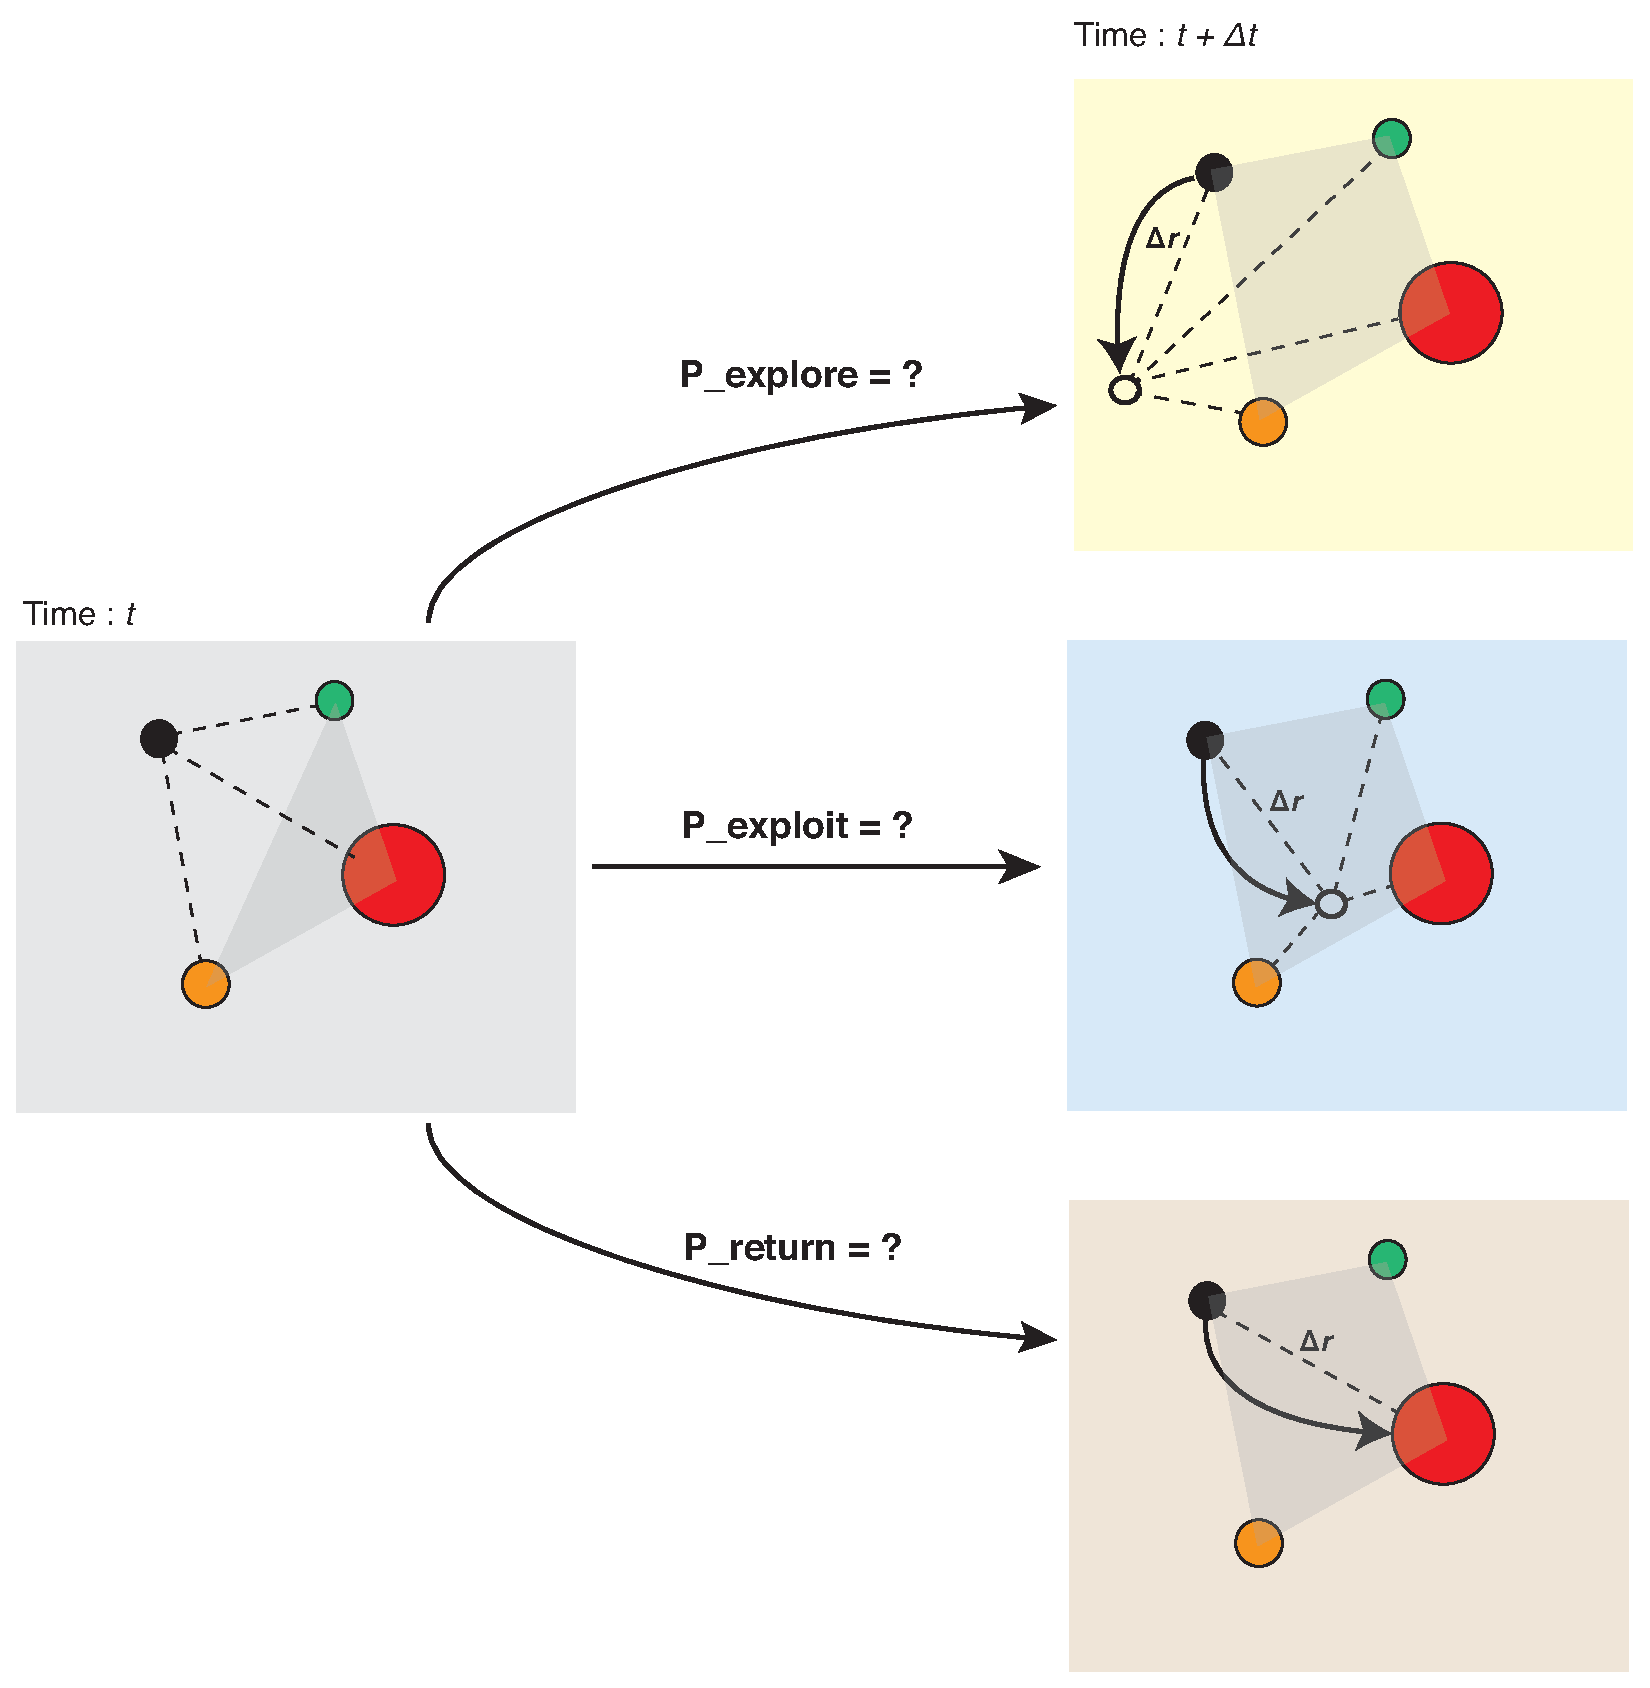
\includegraphics[width=10cm]{figures/schematic_displacement.eps}
\caption{\footnotesize{2-dimensional schematic description of the {\it L\'evy flying mind} model ({\bf ``Proportional Attraction"}): At each time step, the individual must choose between remaining in the solution envelope that has already been explored and exploring outside the currently known solution envelope.  We assign some probability $p$ (a number between 0 and 1) to the participant's decision of staying in the explored envelop and probability $1-p$ to the decision to explore outside that envelop.  If it is harder to find solutions that offer a balanced re-combination of previous solutions than to think out-of-the-box and propose solutions outside of the current solution envelope, then $p < \frac{1}{2}$ else $p \geq \frac{1}{2}$.}}
\label{fig:schematic}
\end{center}
\end{figure}

\section{What can we learn from stylised facts regarding timing ?}

\section{Discrete cascading models and recombination of knowledge}




\section{Discussion}
We find that performance (min distance achieved) is associated with the number of distinct sites visited over time. For that, three aspects are critical : First, the number of proposed solutions (translates into the rate of proposed solutions),  Second, the propensity to return to previously visited solutions, and finally, third, the ability to combine previously visited solutions with new, explorative ones, through an exploration vs. exploitation process, combined with a memory function.  The class of statistical models that has been used to describe such process is known as self-exciting Hawkes processes. 

Some empirical puzzles and theoretical directions remain to be explored. 
In our data we document that with time, mean square displacement decreases, which is another way to say that our participants' solutions improve: This can be due to (i) space limitations, so that their models improve only by chance, which we consider unlikely, (ii) convergence toward the true model, or (iii) stickiness, or, most likely (iv), (ii) and (iii) together.
  
Further, we seek to connect the cascades, described by our data and by the Hawkes processes which describe our data and the human memory giving rise to those data with evolutionary theories and cognitive science about the links between cascades and increased success (resp. counter-performance).  What are the proximate and ultimate causes that move our cognitive and behavioral patterns to follow these strange processes? Next, we will examine the time periods between return visits to past solutions.  If returns are clustered closely in time then they would have much less of an effect on performance than if they are more spread out over time.  


%- connect results with Distance Decay, but basically a model could be summarized as $Distance \sim S_T$ (by the way $D_{min}$ versus $S_T$ could be improved by looking at $D_t$ versus $S_t$). $S_T$ (resp. $S_t$) is a function of displacement $\Delta r$ decisions (which may also cost additional time) and (obviously) their influence on score. 

In summary, at different points in time, a participant must make decisions about displacement, with a part of ``risk", which may be discounted by time spent (waiting time relative to avg waiting time and/or experimentation duration and/or time left). Large displacements may be associated with riskier exploration and more time required for decisions. There exists a $\Delta r$ which maximizes improvement ($\Delta r \approx 0.15$). This suggests that such move size maximizes the chance that a new point in the abstract space will be visited.














\section{Conclusion}


\clearpage
\section{The Experiment} 

Our data comes from an experiment which we conducted at Columbia University's Social Science laboratory.  Participants were given a graphical environment in which they could express their exact believes with respect to the causal structure and probabilistic relationships between 3 or 4 related binary variables, depending on treatment.  Participants were compensated according to their predictions and their predictions' congruence with a series of realizations.  Participants were enabled to dynamically update their models.   The incentives to make good predictions were determined according to an incentive scheme that is standard in experimental economics known as the Becker–DeGroot–Marschak method.  The method implies a quadratic loss function. 

\section{Experimental Design and Implementation}

\subsection{Causal Reasoning about a set of Binary Variables}

Here, we describe and informally define the kinds of systems that experimental participants reasoned about as they participated in our experiment on causal reasoning. 

%\subsubsection{The noisy-or operator \citep{Pearl88}}

%For systems with only binary variables we might think of causation in the following way as suggested by Judea Pearl in 1988.  If causation only involves 2 variables, say $A$ and $B$, where $A$ has a positive causal effect on $B$, then things are simple:

%$P(B = 1 | A = 1) = p$, where $p \in [0, 1]$ and 0 otherwise.  That is, if the cause is present, $B=1$ follows with probability $p$, else it never happens, as there is only one possible cause for $B$ to assume the value $1$ and that is for $A$ to assume the value $1$. Note that in reverse this will mean $P(A=1|B=1)=1$. $B$ can only assume the value $1$ when $A$ is $1$ and thus observing that $B$ is $1$ tells us that $A$ must be $1$ as well. The cookies are gone and there was only one person here who could have eaten them! 

%Other definitions have it that a causal effect of A on B is positive if $P(B = 1 | A = 1) > P(B = 1 | A = 0)$ and $P(B = 0 | A = 1) < P(B = 0 | A = 0)$, but that suggests that there are some ommitted causes of the event $B=1$. 

%Keeping with Judea Pearl's 1986 reasoning, we ask how best to think about causation when there are two binary causes, $B$ and $C$ and one binary outcome. We then generalize this idea. 

%The naive way to pose that would be as:

%$P(A=1|B=b, C=c) = \pi_B*b + \pi_C*c$, 

%where $b, c \in \{1, 0\}$ are the values taken on by the variables $B$ and $C$ and $\pi_B$, $\pi_C \in [0,1]$ are the causal effects of $B$ on $A$ and $C$ on $A$ respectively. But the problem with this formulation -- as Pearl pointed out -- is that, since $P(A=1|B=b, C=c)$ is a probability, as such it must take a value between $0$ and $1$.

%The constraint $0< \pi_B*b + \pi_C*c <1$ induces a dependence between the causal effects $\pi_B$ and $\pi_C$ that we had not explicitly intended in our theory, which posed that $B$ and $C$ each independently cause $A$. Our implicit theory takes the following explicit form \citep{Pearl88}:

%$P(A=1|B=b, C=c) = 1-(1-\pi_B)^b(1-\pi_C)^c$.

%Pearl called it the noisy-OR operator because, supposing $\pi_B=\pi_C=1$, $A$ will be $1$ exactly whenever $B=1$, $C=1$, or both.  When $\pi_B, \pi_C \in (0, 1)$, the OR operator is noisy. The noisy-OR operator accommodates negative causation and any finite number of causes: 

%$P(A=1|B=b, C=c, D=d) = 1-(1-\pi_B)^b(1-\pi_C)^{1-c}(1-\pi_D)^d$,

%where the exponant, $1-c$ in the term $(1-\pi_C)^{1-c}$ means that the variable $C$ exerts a negative causal influence on the variable $A$.

%For a set of binary variables, then, this simple system defines a causal grammar that allows us to construct almost arbitrary causal structures relating the members of the set.  The only constraint is that one may not propose a model with causal cycles. Such models are logically incoherent, unless we allow for dynamics which we don't in this experiment. Here we're going to restrict ourselves to cases where there are no dynamics, there is just a process that repeats in time, like the proverbial coin flip, but with more or less intricate (complex) internal structures.

\subsection{Experimental Treatments}

Data from probabilistic causal systems can be simulated and presented to people so that they may backward engineer the causal structures that generated the patterns that they see. That is, experimental participants see data and build causal models, seeking to understand how the data was produced and to make predictions of future observations. 

To make things more intuitive, we labeled the variables with names from economics, as these seem to relate to many people: "Interest Rate (IR)", "Financial Sector (FS)", "industry (ID)" and "Consumer Spending (CS)". 

%As a side note, it would be interesting so see how labeling could affect learning and diversity.  It can for example be postulated and I find it likely that it is hard for certain people to learn certain relationships because of the meaning that is attached to labels.  Note that I did not include "Taxes" as a variable lable, as this label is a likely candidate to induce hard learning.    

We thus simulated from the joint distributions of two such systems, one simpler and the other more complex and presented people with the data and the modeling tools to learn the causal relationships and parameter values in these systems. The simpler system has three variables: "Interest Rate (IR)", "Financial Sector (FS)" and "Industry (ID)", where the "Interest Rate" has a negative effect on the "Industry" and the "Financial Sector" has a positive effect on the "Industry" (our somewhat arbitrary settings).

For the simple treatment, the data that the participants observed were generated in the following way: a variable was chosen at random from the system's variables to be the current period's "betting variable". The value of this variable was hidden from the participants until the end of the period. Participants were incentivised (on hand the well known Becker–DeGroot–Marschak method) to predict the value of this variable. Next, the value of the "interest Rate" variable was drawn; "H", with probability $0.5$ and "L: with probability $0.5$, followed by the value of the "Financial Sector" variable, with identical probabilities. Lastly, the value of the "Industry" variable was drawn according to Judea Pearl's \citep{Pearl88} probabilistic-OR operator, which gives the conditional probability:  

$P(ID=1|FS=fs, IR=ir) = 1-(1-\pi_{FS})^{fs}(1-\pi_{IR})^{1-ir}$, where we set $\pi_{FS}=\pi_{IR}=0.5$. 


The more complex system had four variables labeled "Interest Rate (IR)", "Financial Sector (FS)", "Industry (ID)" and "Consumer Spending (CS)", where as before the "Interest Rate" has a negative effect on the "Industry" and the "Financial Sector" has a positive effect on the "Industry". In addition, in this system the "Industry" and "Interest Rate" also affect "Consumer Spending". "Industry" positively and the "Interest Rate" negatively.  Please do not hold us accountable for those choices, we will not defend these particular configurations in any way.

The joint distributions of Bayesian Belief Nets can be calculated as the products of the conditional probabilities and the marginal probabilities, as follows. For any number of related variables, $X_1, \ldots, X_n$, their joint probability can be calculated as:

$P(x_1, \ldots, x_n) = P(x_1 | x_2, \ldots, x_n)*P(x_2 | x_3, \ldots, x_n)*\cdots*P(x_{n-1} |x_n)*P(x_n)$.
\\

$P(x_1, \ldots, x_n) = P(x_1 | x_2, \ldots, x_n)*P(x_2 | x_3, \ldots, x_n)*\cdots*P(x_{n-1} |x_n)*P(x_n)$.
\\

For example, remembering that $P(ID=1|FS=fs, IR=ir) = 1-(1-\pi_{FS})^{fs}*(1-\pi_{IR})^{1-ir}$, where $\pi_{FS}=\pi_{IR}=0.5$, for the simple treatment, the joint outcome $FS=H, IR=H, ID=H$ has probability:
\\

$P(FS=H, IR=H, ID=H) = P(ID=1|FS=H, IR=H)*P(FS=H)*P(IR=H)=\left(1-(1-\pi_{FS})^{1}*(1-\pi_{IR})^{1-1}\right)*0.5^2 =0.125.$  
\\

A frequentist, might simply count membership of the joint buckets and build a model that matches the percentages. Updating her beliefs in this context of a repeating process, a Bayesian could essentially do the same thing by comparing members of the Dirichlet distribution class (for example, depending on priors) by observing, updating and finding the maximum of the posterior distribution of the parameters, known as the pseudo counts. This maximum turns out to approach the $2^k$ dimensional value of the bin counts. Likewise, all conditional distributions could be calculated in this way, but cognitive scientists and computer scientists have recently found this to be computationally more expensive than necessary \citep{Griffith08, Koller03}.  They suggest that instead of calculating $2^k$ parameters for the joint distribution of $k$ binary variables, people and computers should build structural models, where they can update their beliefs for a much reduced number of parameters and obtain the same results. For the model that we used as the simple treatment process, for example, if one has the right structure and the correct idea that $P(ID=1|FS=0, IR=1)=0$, there are four parameters to form beliefs about: $\pi_{FS}, \pi_{IR}, P(FS), P(IR)$. But perhaps, one doesn't see causation in that way and then there are $5$ parameters.  The full joint distribution has eight parameters.  There are thus less parameters to estimate if a causal theory is postulated. The benefit of thinking structurally will increase as the number of variables gets large because most often, the number of causal relationships (structural parameters) increases linearly in the number of variables, $k$, whereas the parameters of the joint distribution increases exactly by $2^k$.  At most, each variable that is added, affects every variable that is already there and then the number of causal arrows grows with $k$ as $k(1-k)$. In light of this, it seems evident that people should have a harder time guessing the correct structure and estimating the correct structural parameters when the system is complex than when it is simple. This, we hypothesized, should lead their models to be more diverse and less accurate in the complex case. 



\bibliographystyle{apsrev4-1}
\bibliography{bib/references,bib/cognition_causality,bib/levyflight_foraging,bib/misc,,bib/orgsci}

\clearpage
\begin{center}
{\Large {\bf Figures}}
\vspace{1.5cm}
\end{center}
%
%\begin{figure}[h!]
%\begin{center}
%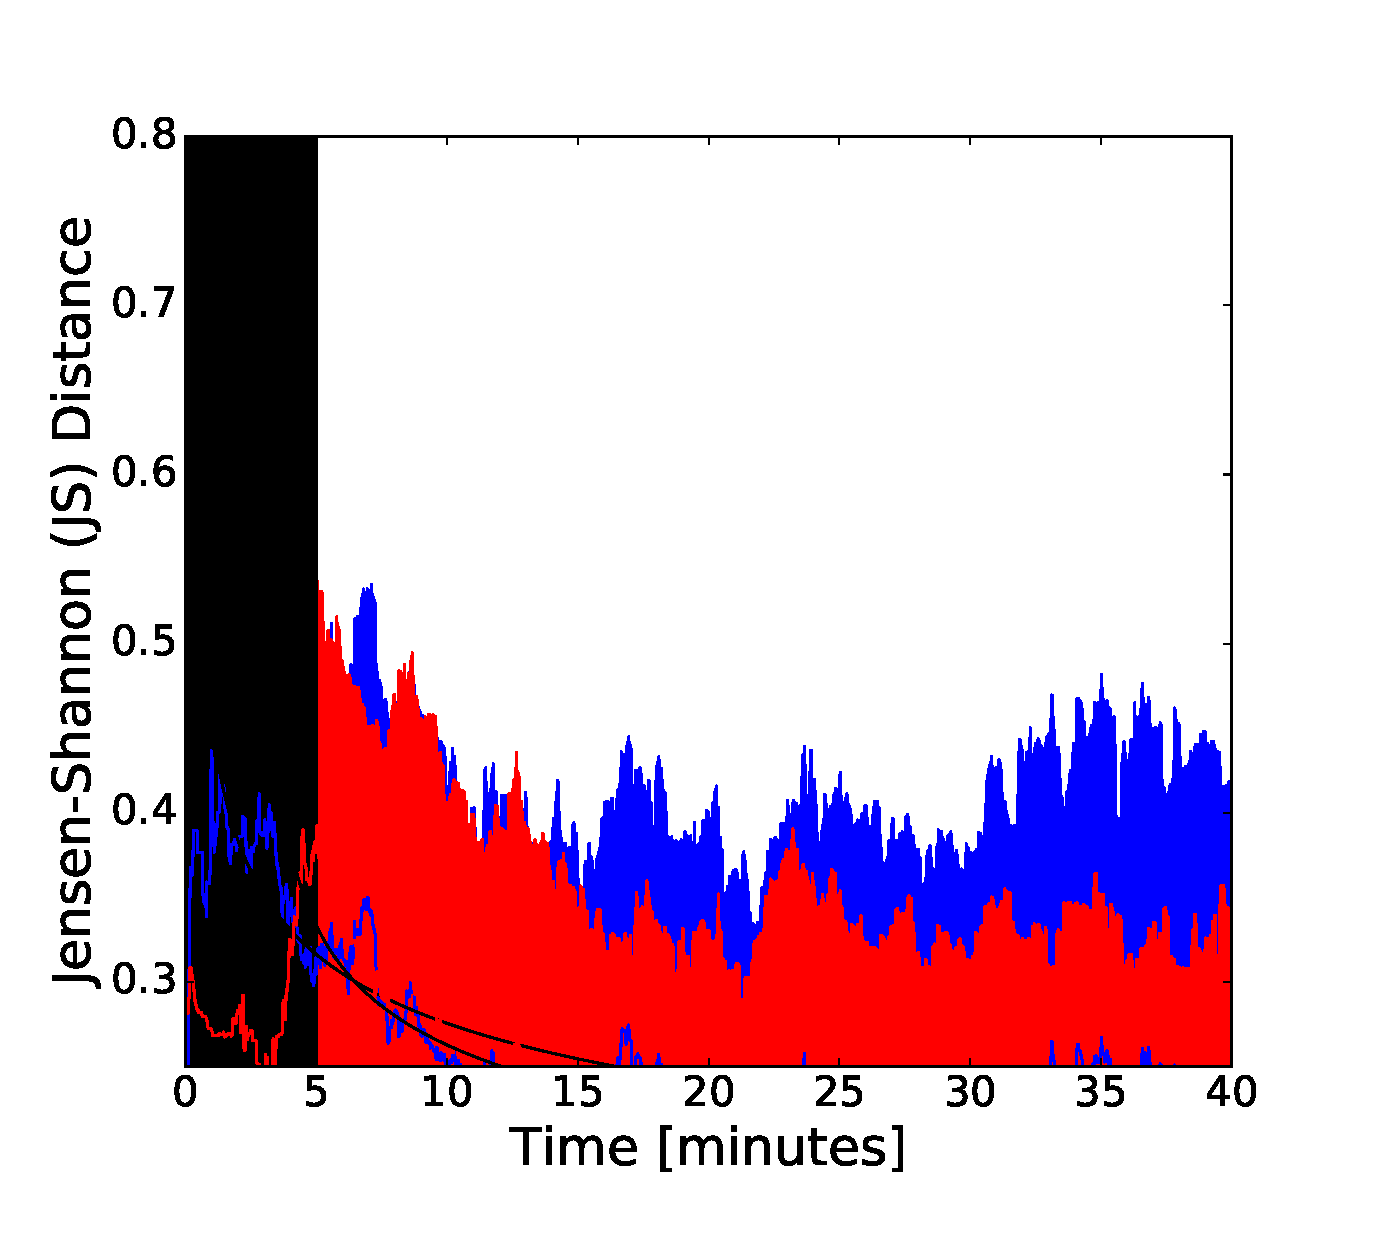
\includegraphics[width=12cm]{figures/decay_simple_complex.eps}
%\caption{\footnotesize Decay of the Jensen-Shannon (JS) Distance (\ref{JS-distance}) between models proposed by participants and the true model over time for the 3-node (simple) and 4-node (complex) Bayesian network treatments (resp. in blue and red). The colored areas show the standard deviation. The decays are averaged (mean) over all participants for each treatment. Both treatments follow similar extremely slow power law decay (\ref{power_law_decay}), yet with different exponents: $\alpha = 0.1$ ($p < 0.001$, $R = -0.92$) for the simple Bayesian network treatment and $\alpha = 0.07$ ($p < 0.001$, $R = -0.94$) for the complex Bayesian treatment. The grey area on the left shows the 5-minute {\it warm up} period during which participants get used to the interface. In both treatments, participants elaborate initial Bayesian Net models with $JSD \approx 0.6$, and there is a phase associated with counter-performance (during which the JS Distance increases). This phase is however much shorter for the simple Bayes Net (peak at $t \approx1$ minute) compared to the complex Bayes Net (peak at $t \approx 4.5$ minutes) after which the JS-distance actually starts to decay.}
%\label{fig:decay}
%\end{center}
%\end{figure}

%\begin{figure}[h!]
%\begin{center}
%\includegraphics[width=15cm]{figures/pdf_JSD.eps}
%\caption{{\bf a.} Probability density function (un-normalized) of $\Delta(JS-distance)$ ($\Delta JSD$) between 2 consecutive changes (jump sizes). The negative $\Delta(JS-distance) < 0$ stands for improvement (i.e., the goal is to reduce the $JS-distance$). On the contrary, the $\Delta(JS-distance) >  0$ happens when a participant comes up with a BayesNet model which is further from the true model, compared to the previous attempt. The distribution is heavy-tailed on both sides (c.f., {\bf b.} and {\bf c.}), almost power law tail, yet with some particularities: For $\Delta JSD < 0$, the probability density function may be a {\bf log-normal}. For $\Delta JSD > 0$, an extra ``outliers" regime is present (grey shade rectangle). Also, $\Delta JSD > 0$ is more heavy-tailed compared to $\Delta JSD < 0$ (see Table \ref{pwlaw_fits}). The {\it simple} and {\it complex} treatments (resp. blue and red dots) look similar, yet with sligtly different exponents (see again Table \ref{pwlaw_fits}). Interestingly, the median in both simple and complex cases is very close to zero [$median(pdf) < 0.001$], which means that on average, after a change was made to a model the model is only a slight improvement over the old.}
%\label{fig:jump_sizes}
%\end{center}
%\end{figure}

\begin{figure}[h!]
\begin{center}
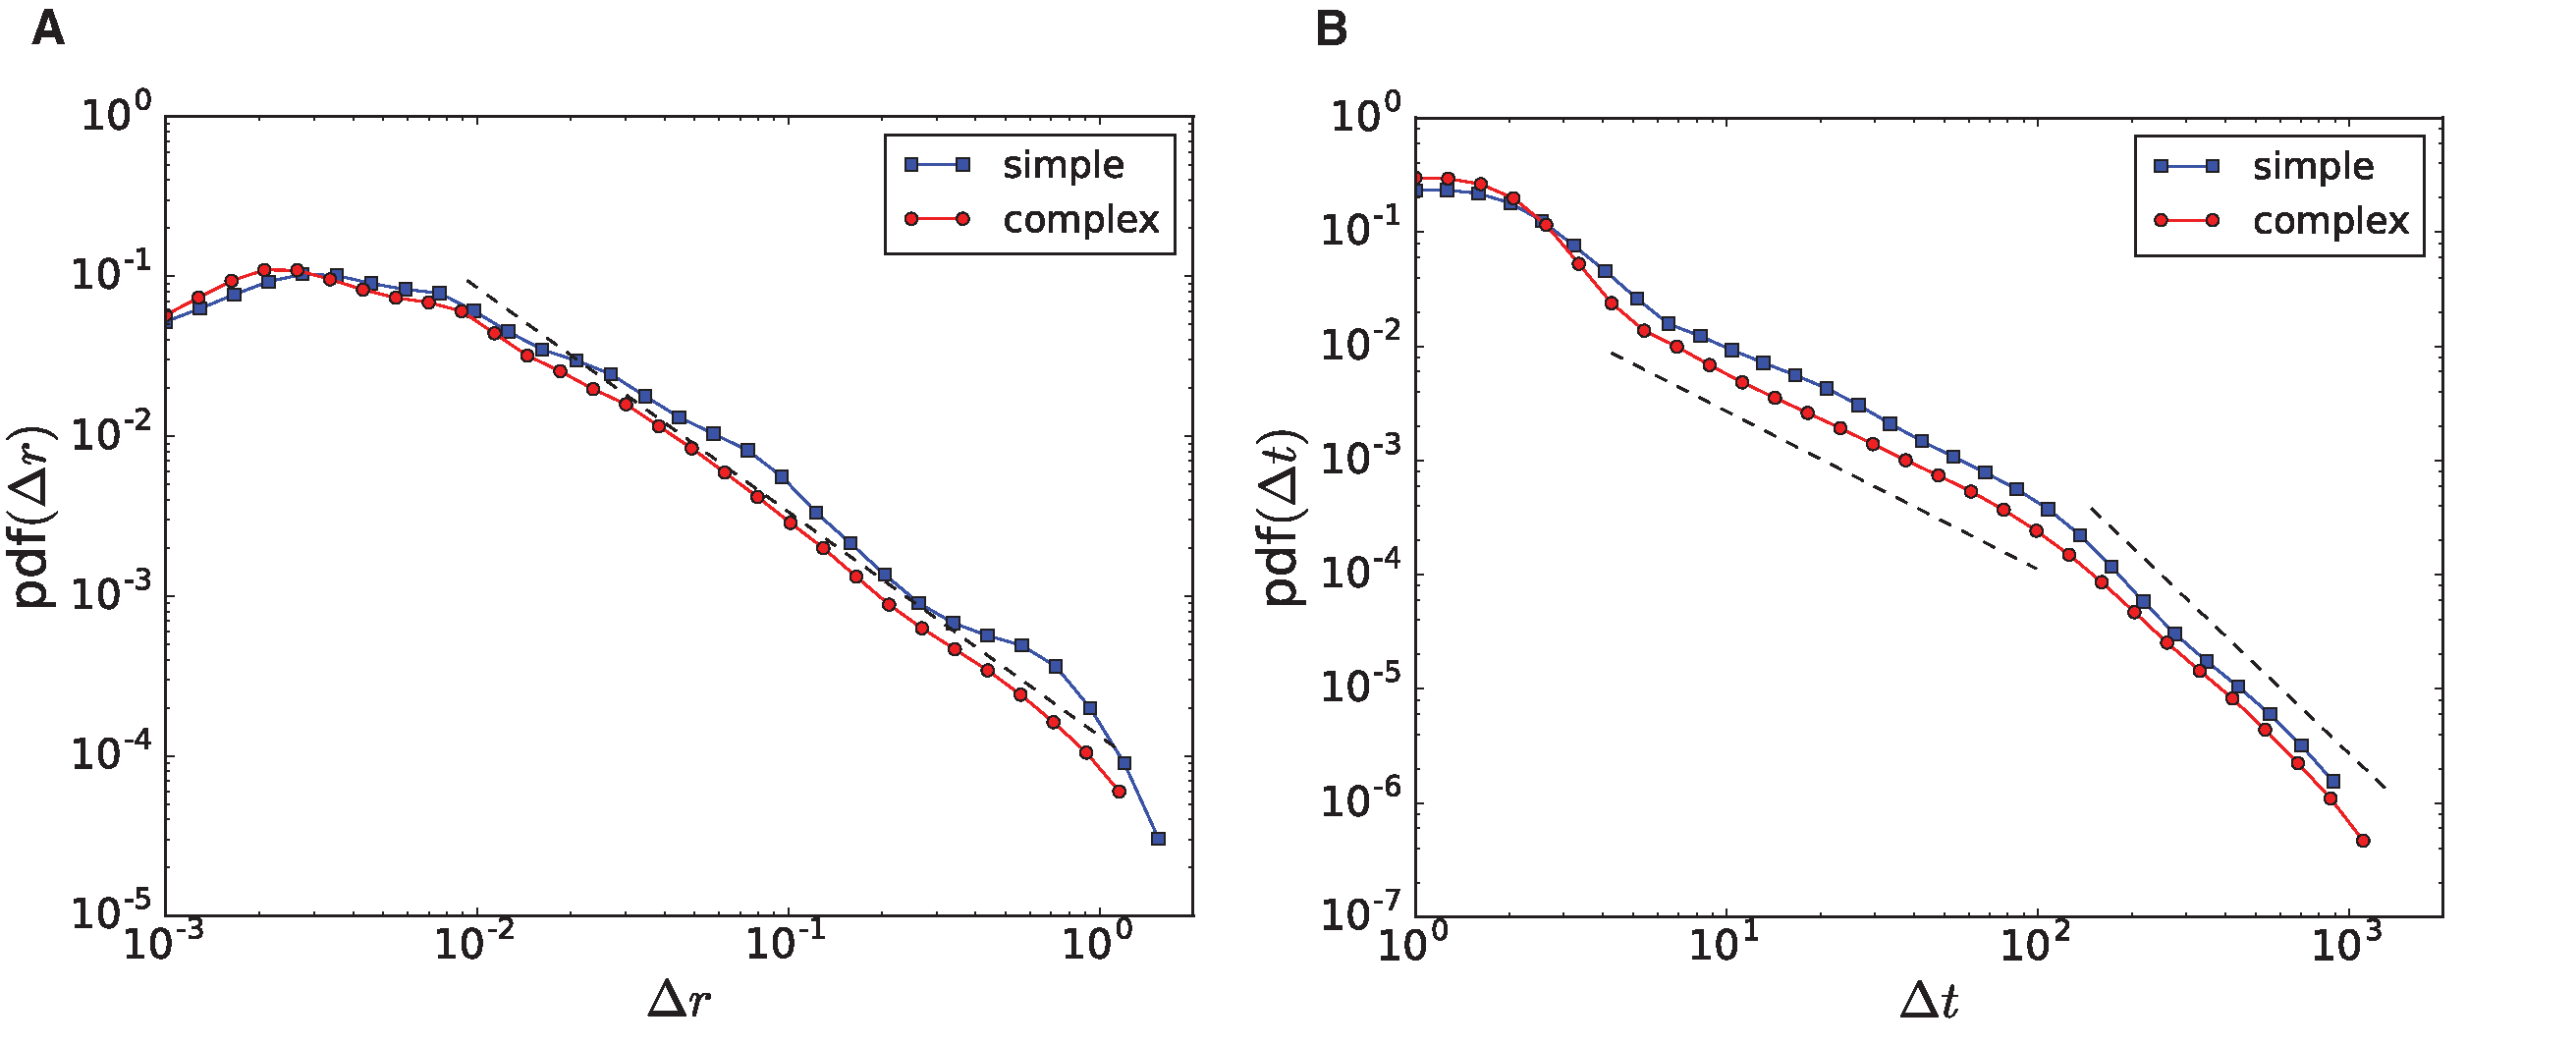
\includegraphics[width=17cm]{figures/pdfs.pdf}
\caption{{\bf A.} Probability density function of displacement $pdf(\Delta r) = \Delta r^{-\alpha -1}$ with $\alpha = 0.40(5)$. {\bf B.} Probability density function of waiting time $\Delta t$ $pdf(\Delta t) = \Delta t^{-\beta -1}$ with 2 regimes : $\beta_{\Delta t < 125} = 0.38(4)$ and $\beta_{\Delta t > 125} = 1.59(5)$. Distributions of $\Delta r$ and $\Delta t$ are equivalent for the simple and complex treatments.}
\label{fig:pdfs}
\end{center}
\end{figure}




%\begin{figure}[h!]
%\begin{center}
%\includegraphics[width=15cm]{figures/ccdf_waiting_time.eps}
%\caption{Distribution of Waiting Times is fairly the same in both the simple and complex cases.}
%\label{fig:waiting_times}
%\end{center}
%\end{figure}

\begin{figure}[h!]
\begin{center}
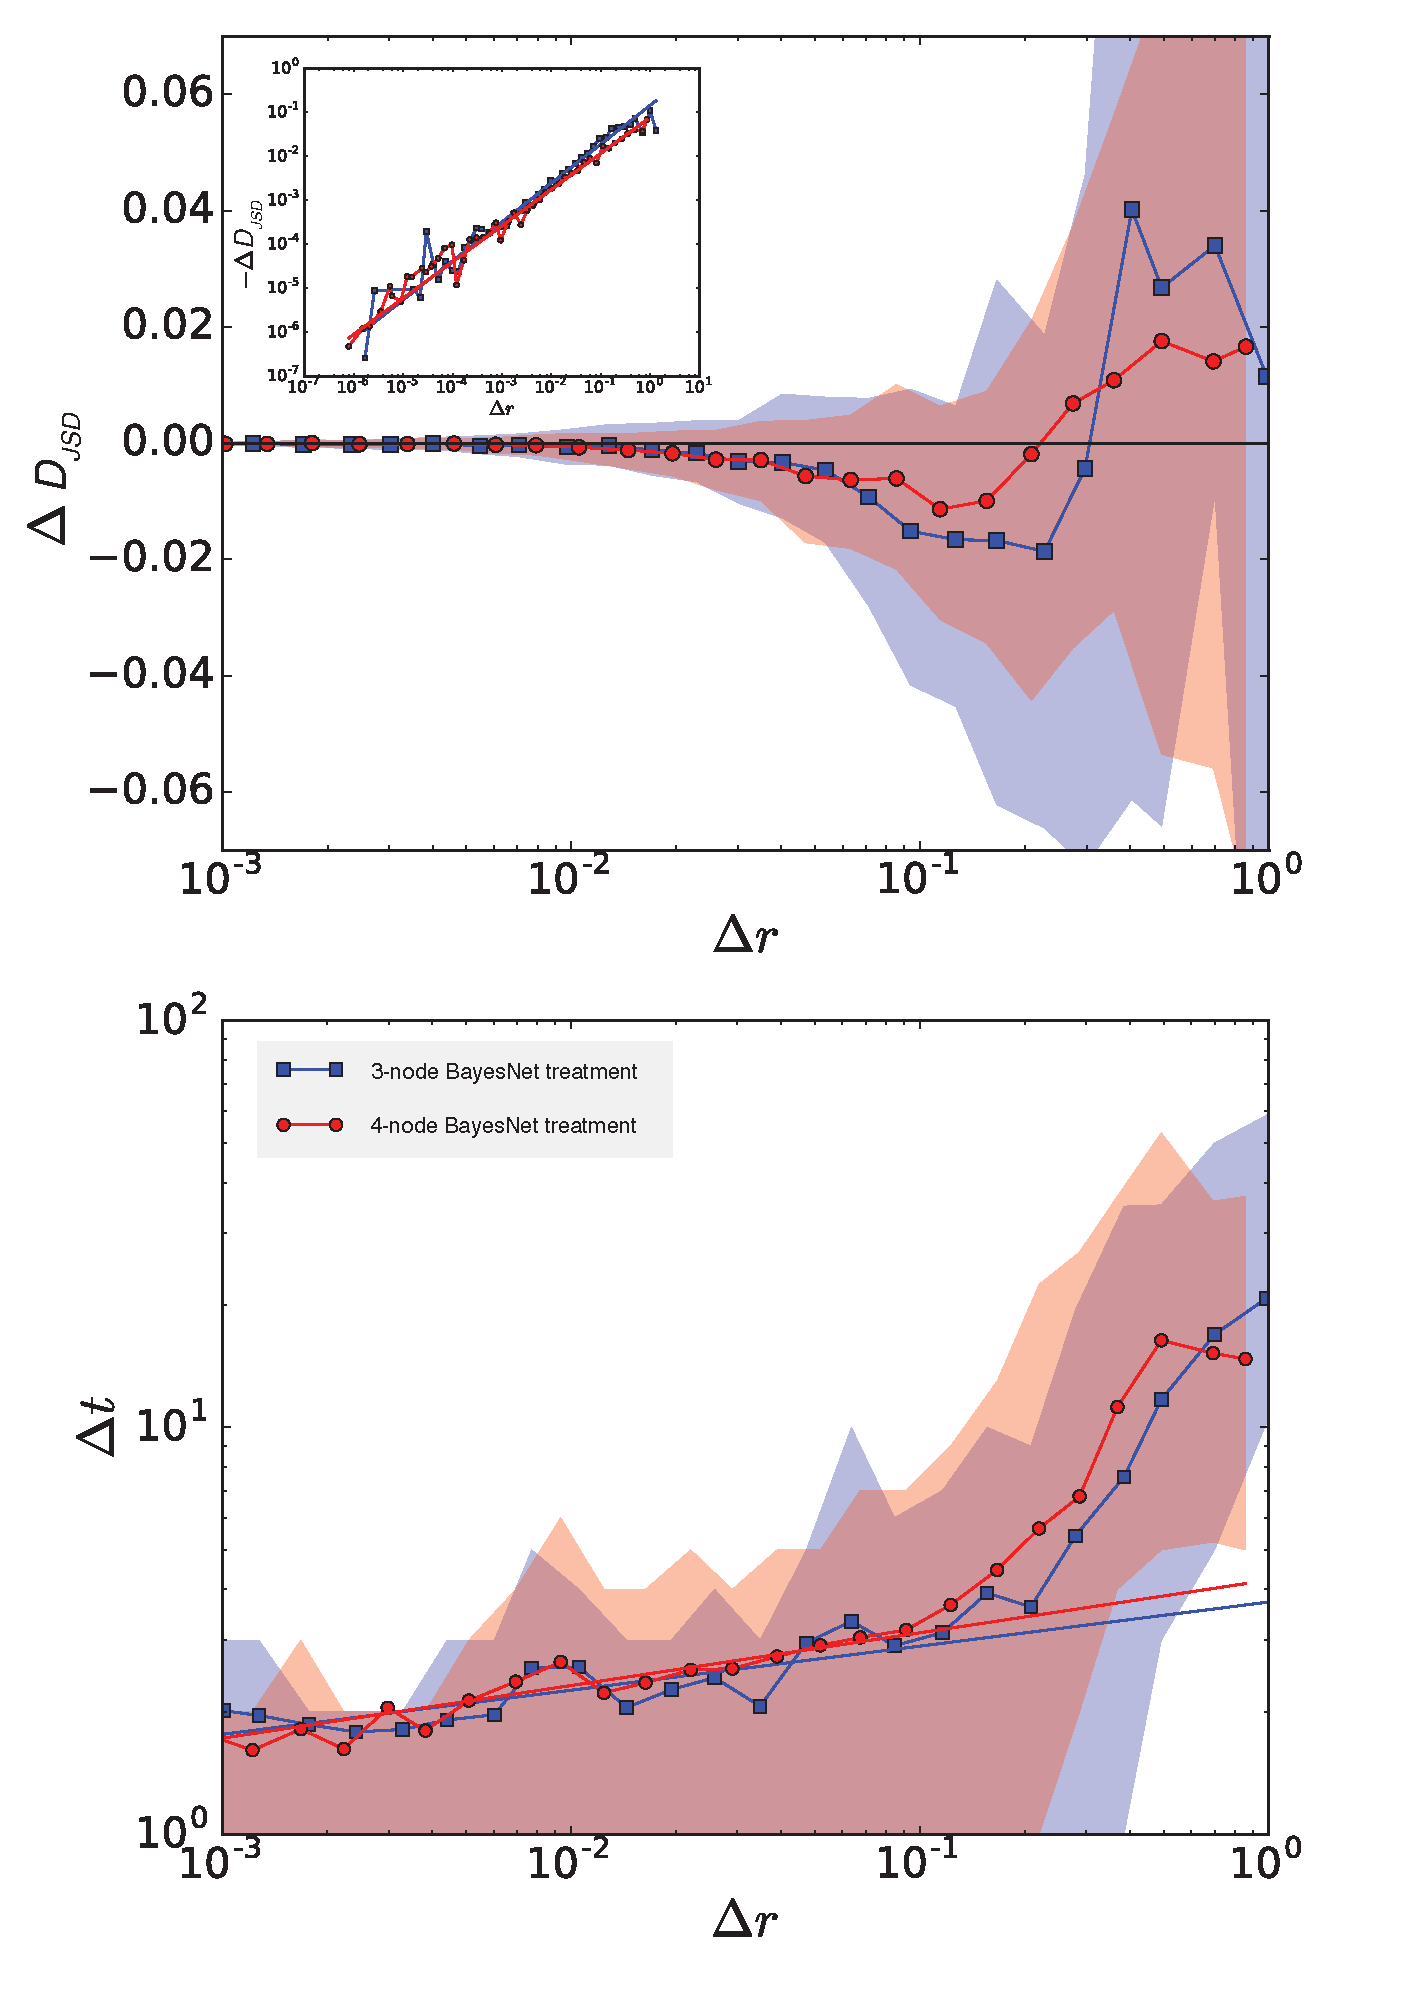
\includegraphics[width=11cm]{figures/vs_dr.pdf}
\caption{{\bf A.} Evolution of the distance to the true model $D$ as a function of displacement $\Delta r$. The distance scales as $D \sim {\Delta r}^{\mu}$ with $\mu_{simple} = 0.88(1)$ [resp. $\mu_{complex} = 082(2)$]. For $\Delta r > 0.2$, $D$ becomes quickly highly uncertain, but rather positive, reflecting the {\it cost} of the making ``wild"displacements. {\bf B} For $\Delta r < 0.2$, the waiting time before a displacement decision is made scales as $\Delta t \sim \Delta r^{\gamma}$ with $\gamma_{simple} = 0.11(1)$ [resp. $\gamma_{complex} = 0.13(1)$]. For $\Delta r > 0.2$, the waiting time before a displacement decision is taken get disproportionally long (up to tens of seconds on average for displacement of 0.7 (i.e., $\approx 25\%$ of the maximum displacement distance). On both panels, blue and red areas show the 25th percentile confidence intervals.}.
%\caption{Scaling relation between $\Delta t$ and $\Delta r$ for the simple (A) and complex (B) treatments. The functions are similar for both treatments [resp. $\sim 0.44(2)$ ($p < 0.01$ , $r = 0.39$) and $\sim 0.47(2)$ ($p < 0.01$ , $r = 0.36$)]. {\bf Actually, one may see this figure differently : scaling $\Delta t \sim {\Delta r}^{0.2}$ for $\Delta r < 0.2$ and another (unknown) regime for $\Delta r > 0.2$ with waiting time getting disproportionately long $\rightarrow$ This may highlight the processing costs associated with a big jump.}}
\label{fig:vs_dr}
\end{center}
\end{figure}


\begin{figure}[h!]
\begin{center}
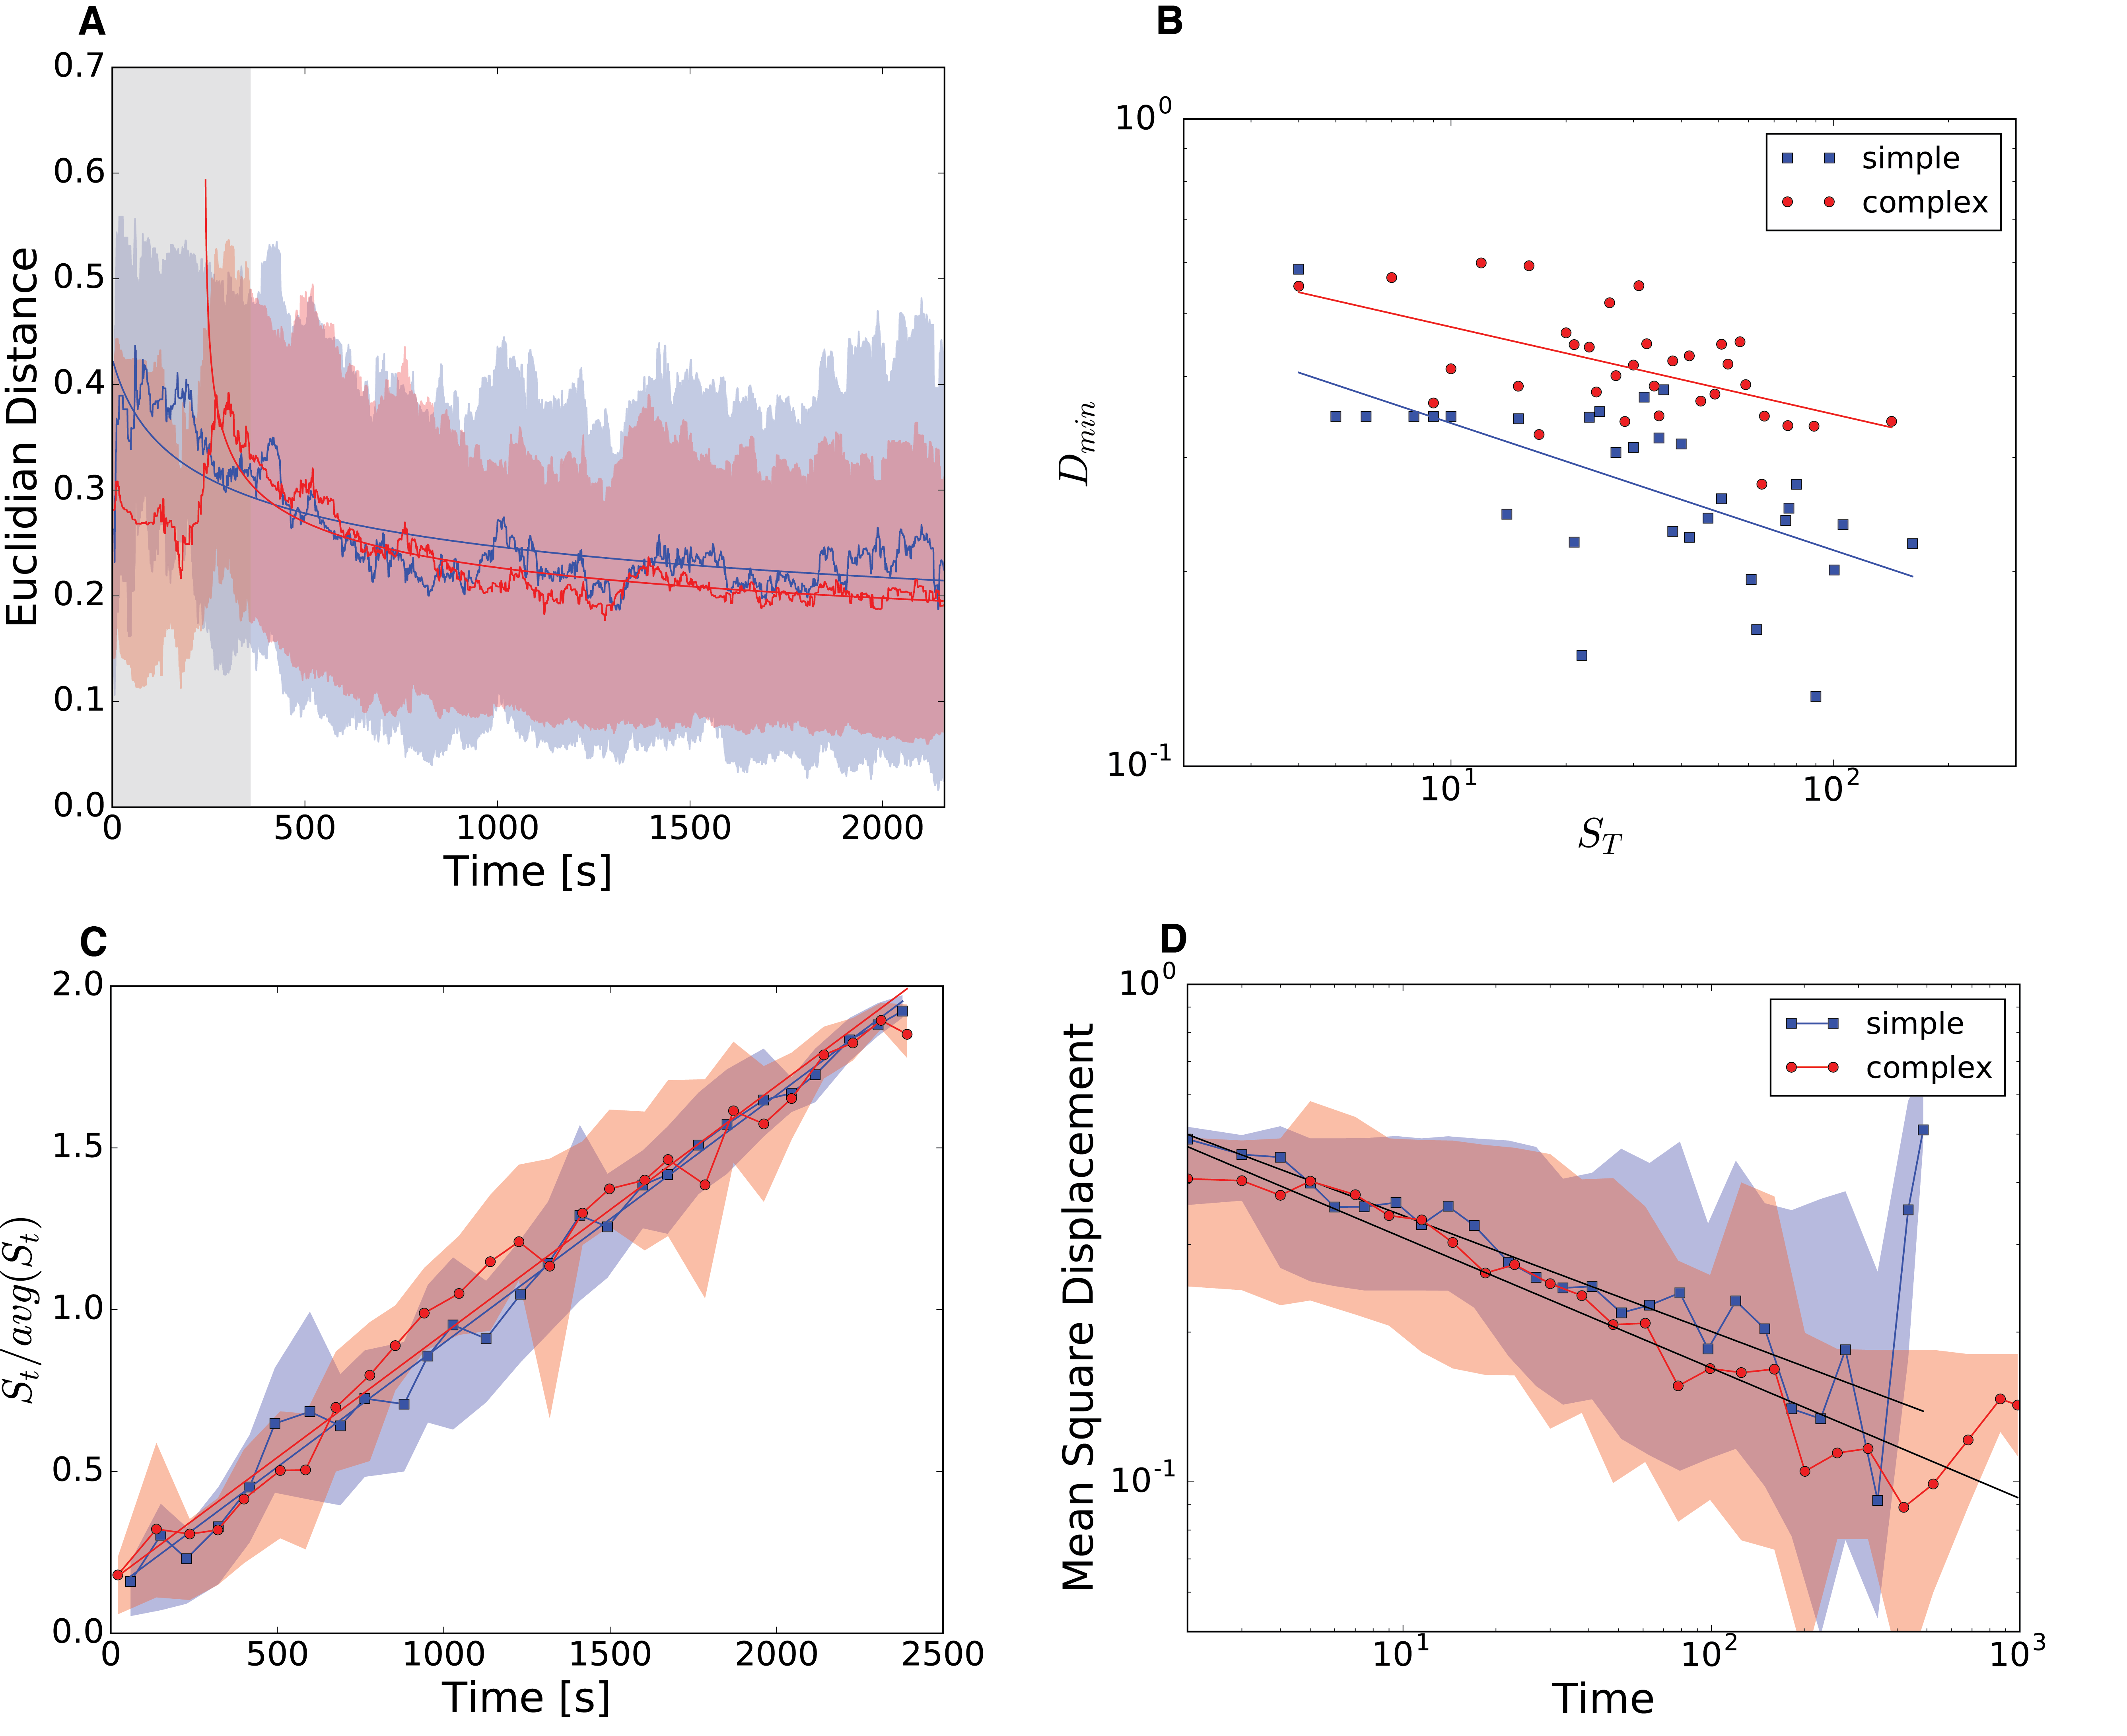
\includegraphics[width=16cm]{figures/Dmin_vs_St.png}
\caption{{\bf A.} Average Euclidian Distance $\langle D \rangle$ decays as function of time as $\sim t^{\nu}$ with $ \nu \approx -0.15(1)$ indicating a very slow convergence to the true model. {\bf B.} Minimum Euclidian distance $D_{min}$ (between the best model and the true model) exhibits a scaling as a function of the number of distinct sites visited $S_{T}$. $D_{min} \sim S_{T}^{\gamma}$ with resp. $\gamma_{simple} = -0.20(4)$ and $\gamma_{complex} = - 0.13(3)$. {\bf C.} The number of visited sites over time $S_t$ is a linear function of time $t$. Hence, the number of distinct visited sites is a predictor of the minimum distance $D_{min}$ achieved. The result also holds for average distance. {\bf D.} Mean square displacement (MSD) decays as $\sim t^{\mu}$ with $\mu_{simple} =-0.23(2)$ and $\mu_{complex} =- 0.26(1)$ showing a slow convergence (on the contrary of a normal L\'evy flight / CTRW, which is characterized by respectively diffusion $\mu_{Levy} = 1$ or super-diffusion $\mu_{CTRW} = \beta$ \cite{21,23}). All colored areas show the 25th percentile confidence intervals.}
\label{fig:Dmin_vs_St}
\end{center}
\end{figure}



\begin{figure}[h!]
\begin{center}
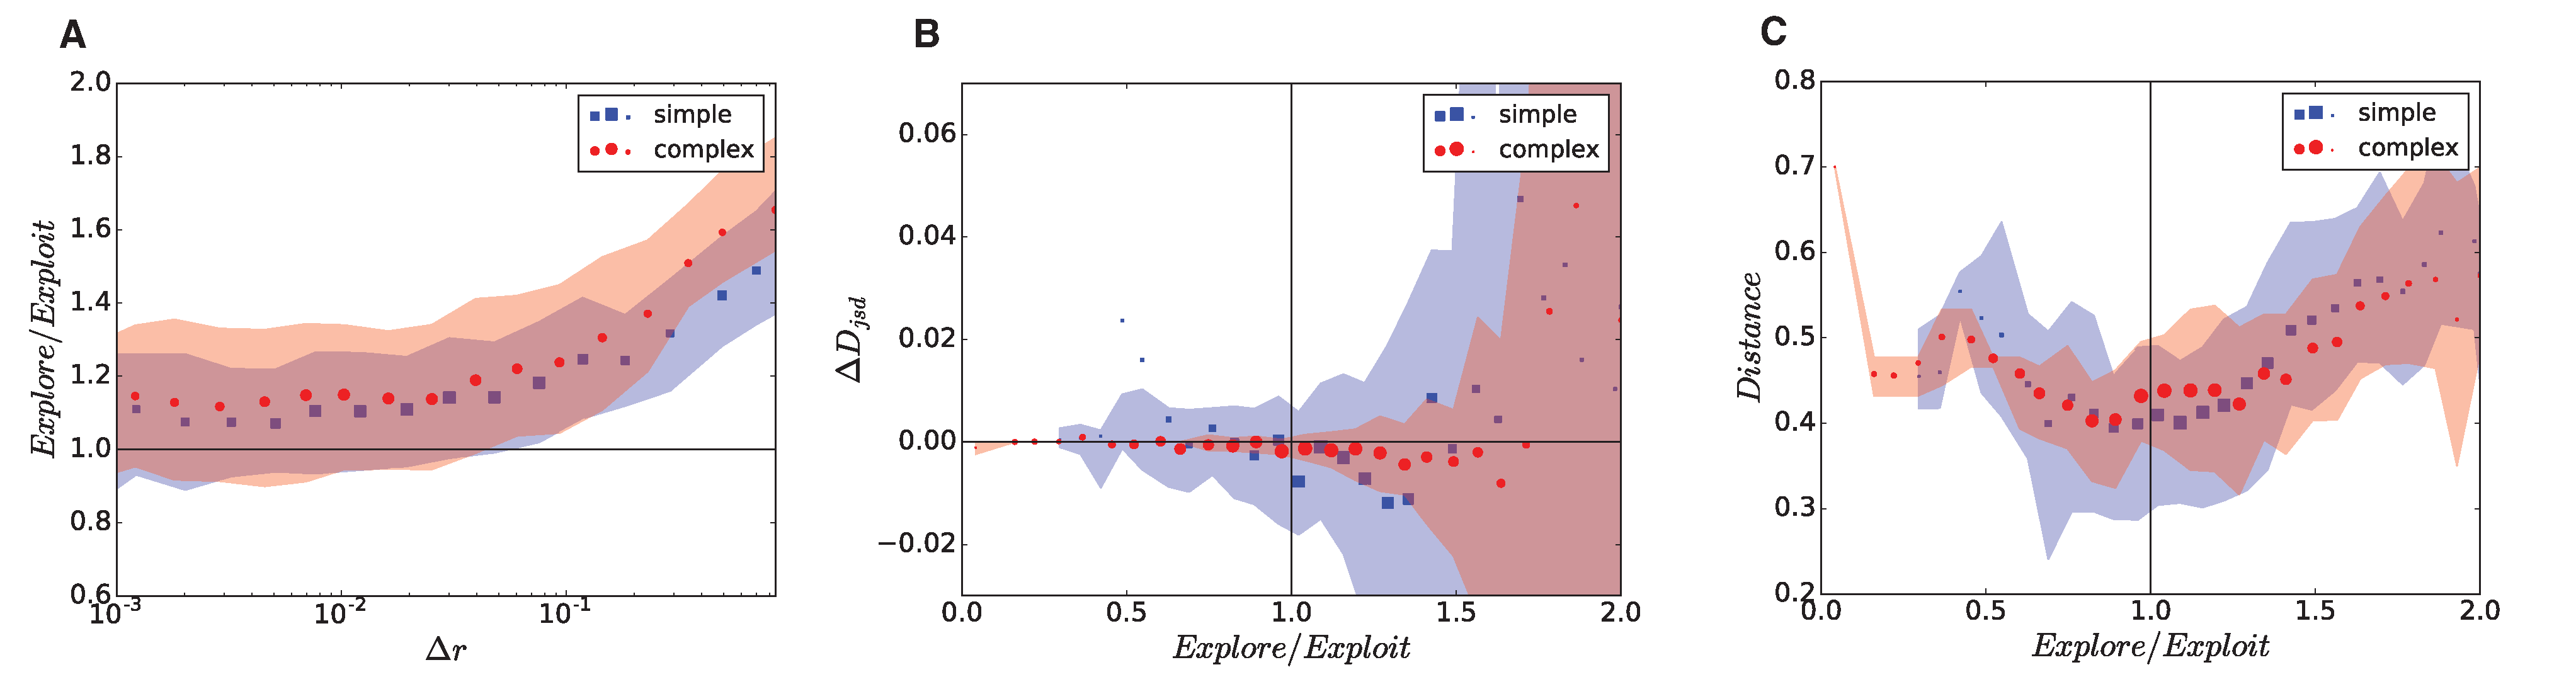
\includegraphics[width=18cm]{figures/EE.eps}
\caption{{\bf A.} Explore / Exploit ($EE$ )as a function of displacement $\Delta r$. {\bf B.} $\Delta D_{jsd}$ as a function Explore / Exploit: Improvement seems better for $EE \approx 1.4$. {\bf C.} $D_{jsd}$ as a function of $EE$: As distance gets smaller, a balance around $EE = 1$ seems to be reached.}
\label{fig:pdf_return}
\end{center}
\end{figure}

\begin{figure}[h!]
\begin{center}
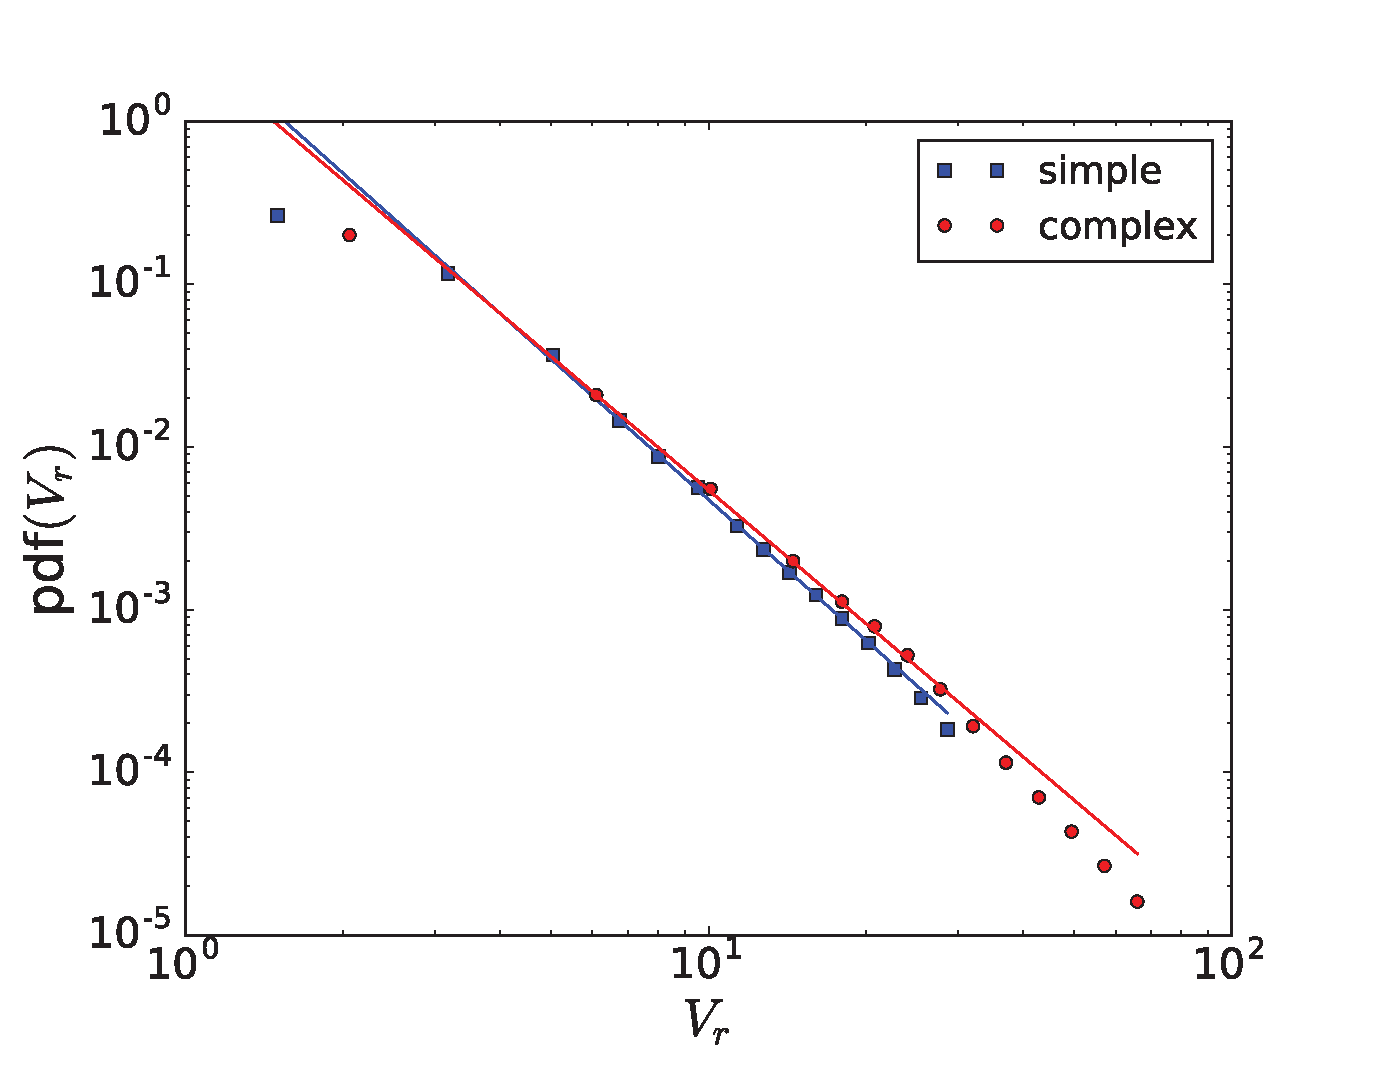
\includegraphics[width=10cm]{figures/pdf_return.eps}
\caption{return to previously visited sites : $\mathrm{pdf}(V_r) \sim {V_r}^{- \gamma -1}$, with $\gamma_{simple} = 1.6(1)$ and $\gamma_{complex} = 1.5(1)$ $\rightarrow$ tendency to return to previously visited sites : This goes against the imperative to visit new sites (maximize $S_T$) in order to reduce $D_{min}$ (c.f. Figures \ref{fig:Dmin_vs_St}B and \ref{fig:Dmin_vs_St}C). Moreover, given the large number of sites [$10^{8}$ (resp. $10^{16}$) in the simple (resp. complex) case], it is remarkable that participants tend to return to exactly the same (tiny) spots. This suggest some stickiness of memory.}
\label{fig:pdf_return}
\end{center}
\end{figure}




\begin{figure}[h!]
\begin{center}
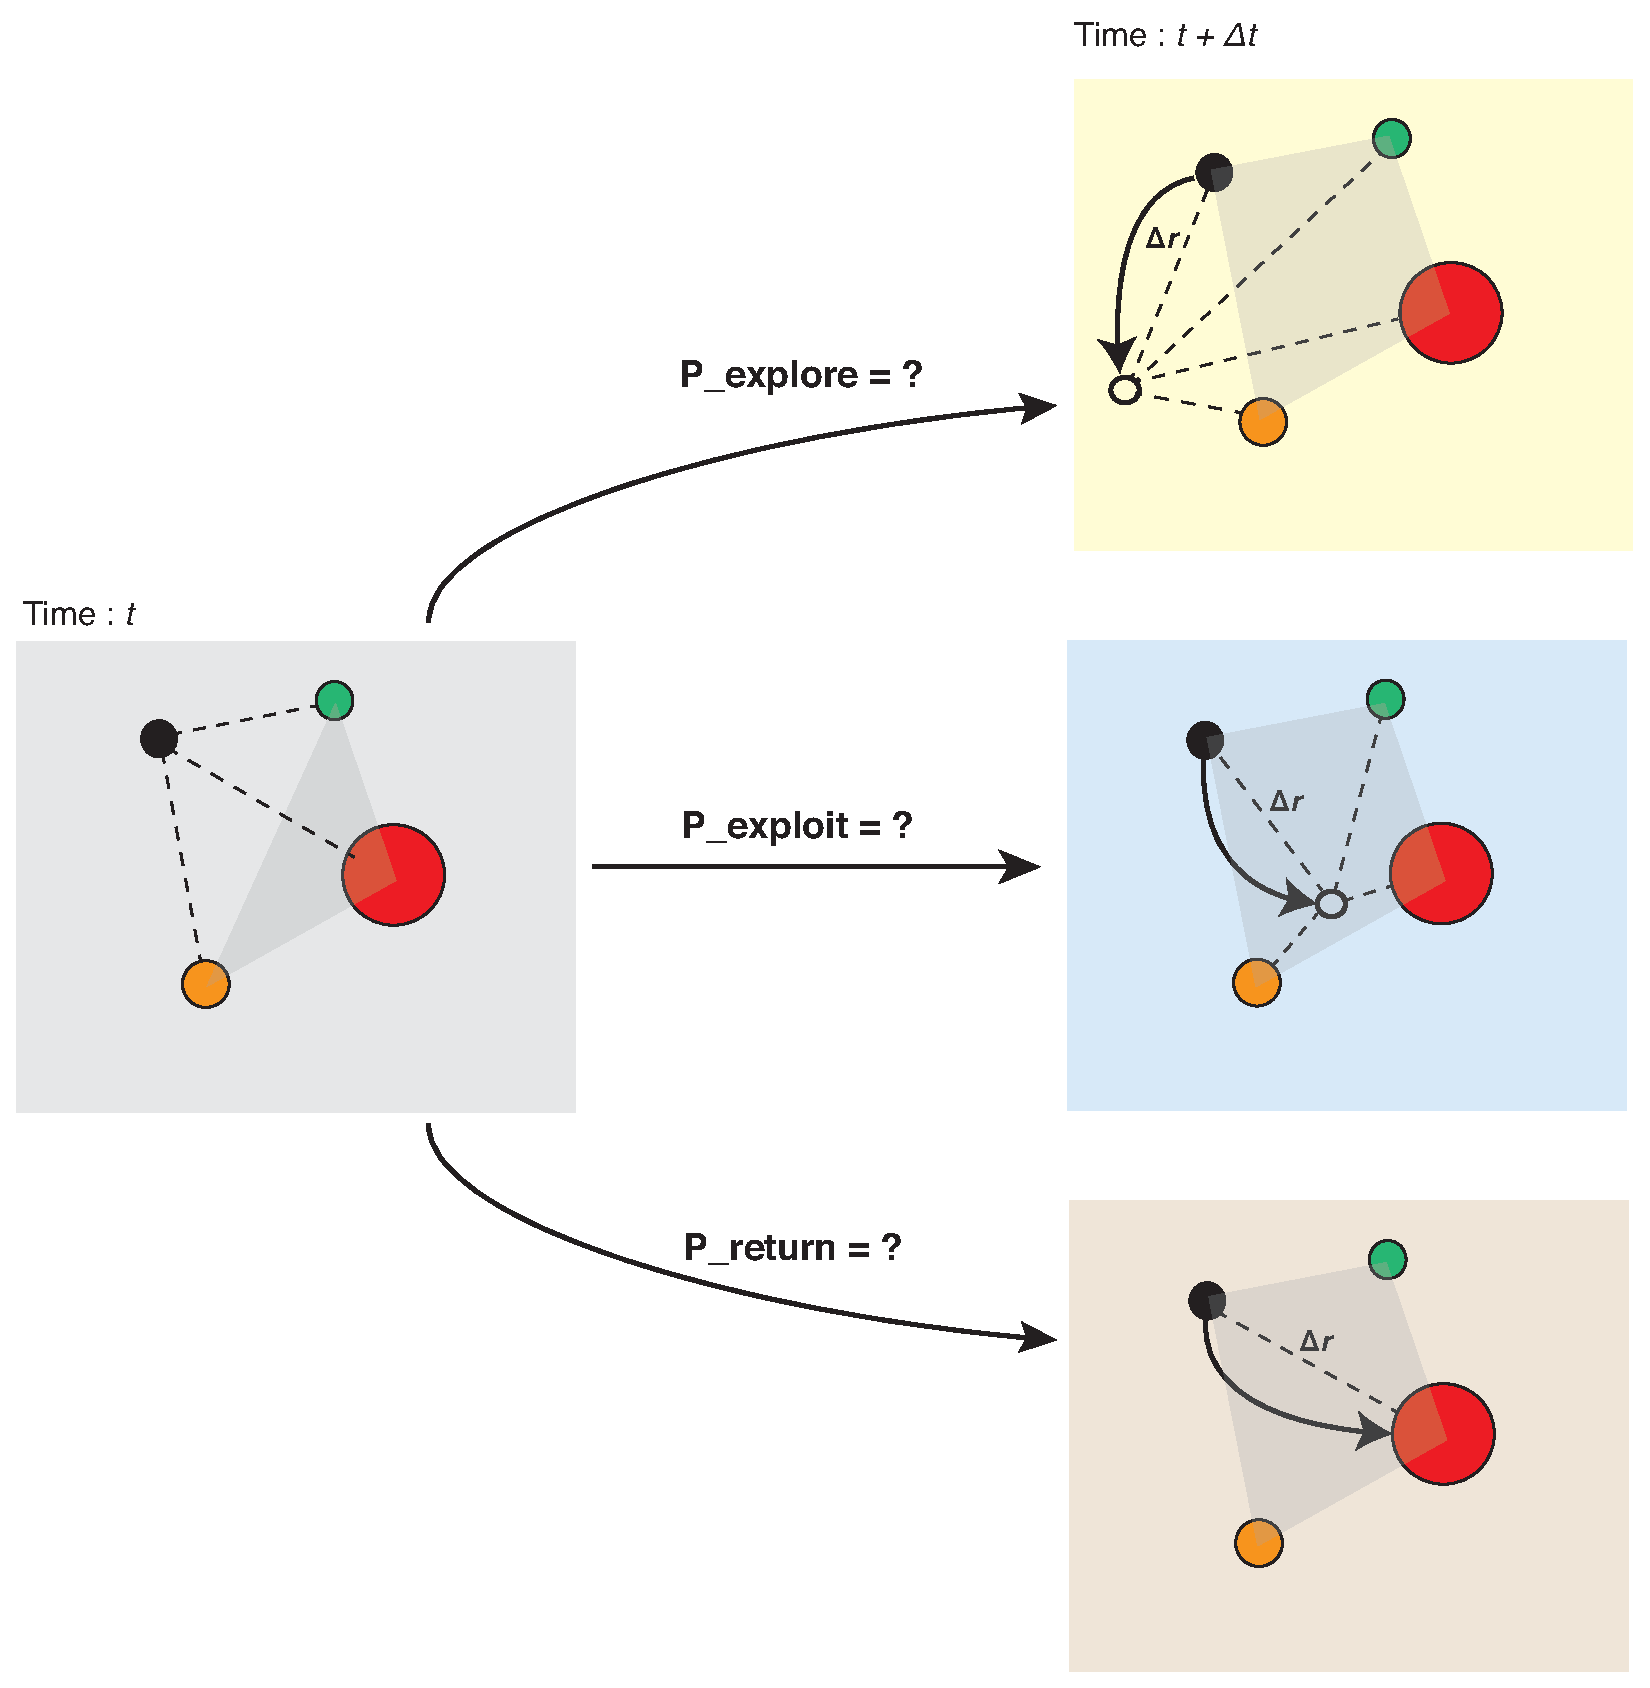
\includegraphics[width=12cm]{figures/schematic_displacement.eps}
\caption{2-dimensional schematic description of the {\it L\'evy flying mind} model ({\bf ``Proportional Attraction"}): At each time step, the individual must choose between remaining in the solution envelope that has already been explored and exploring outside the currently known solution envelope.  We assign some probability $p$ (a number between 0 and 1) to the participant's decision of staying in the explored envelop and probability $1-p$ to the decision to explore outside that envelop.  If it is harder to find solutions that offer a balanced re-combination of previous solutions than to think out-of-the-box and propose solutions outside of the current solution envelope, then $p < \frac{1}{2}$ else $p \geq \frac{1}{2}$.}
\label{fig:schematic}
\end{center}
\end{figure}

%\begin{figure}[h!]
%\begin{center}
%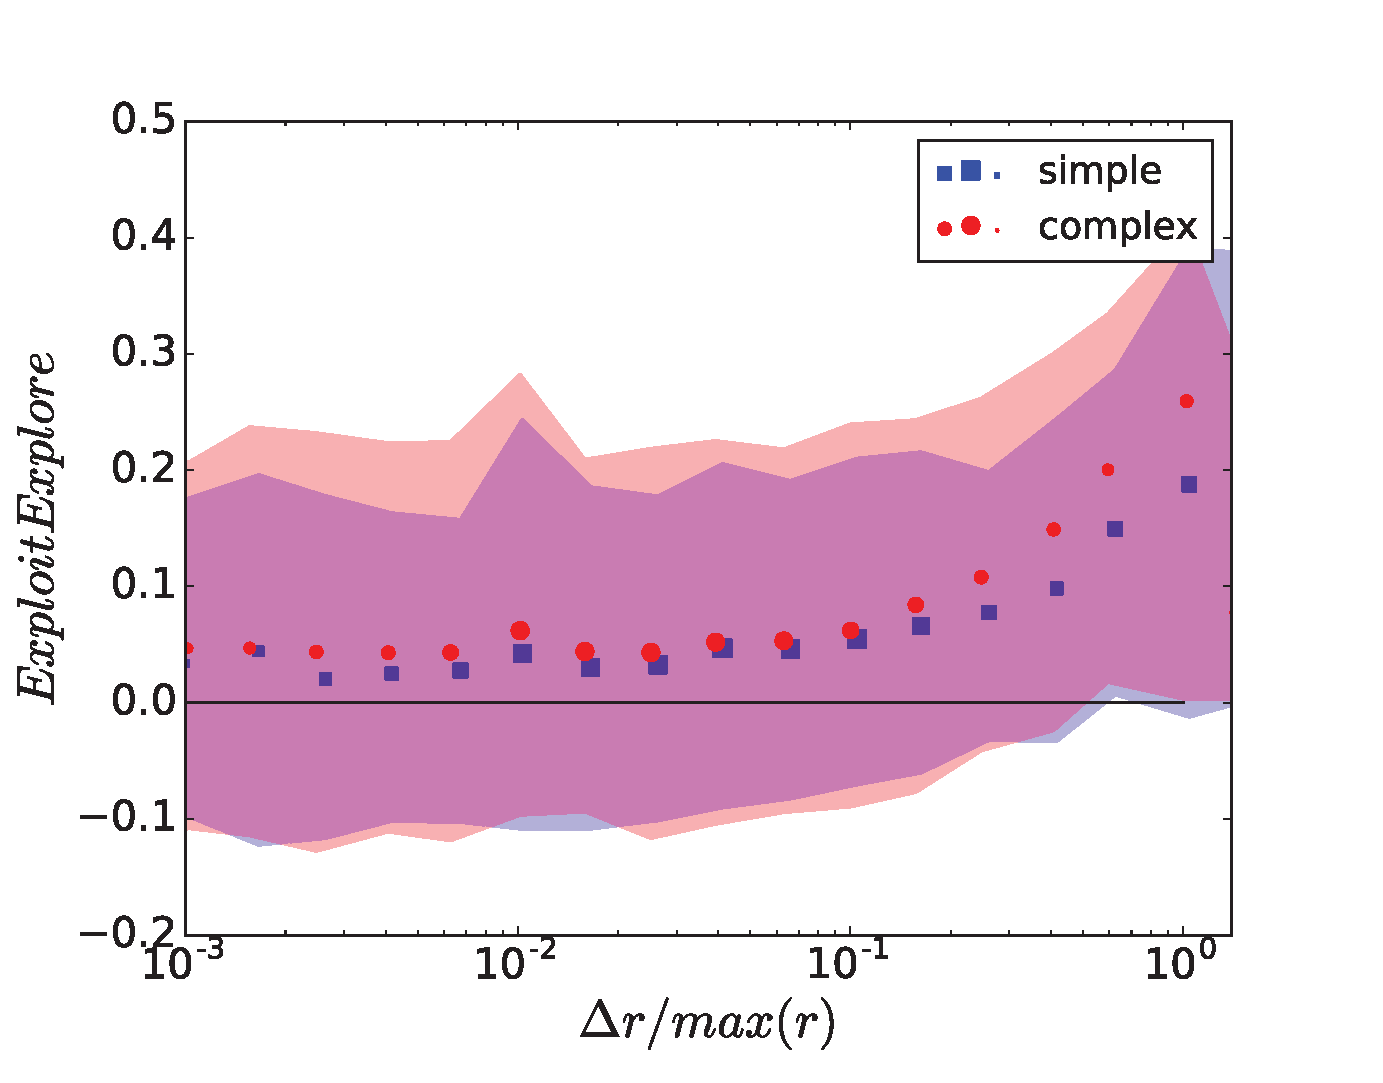
\includegraphics[width=13cm]{figures/EE_vs_Dr.eps}
%\caption{explore exploit}
%\label{fig:exploit_explore}
%\end{center}
%\end{figure}



\begin{figure}[h!]
\begin{center}
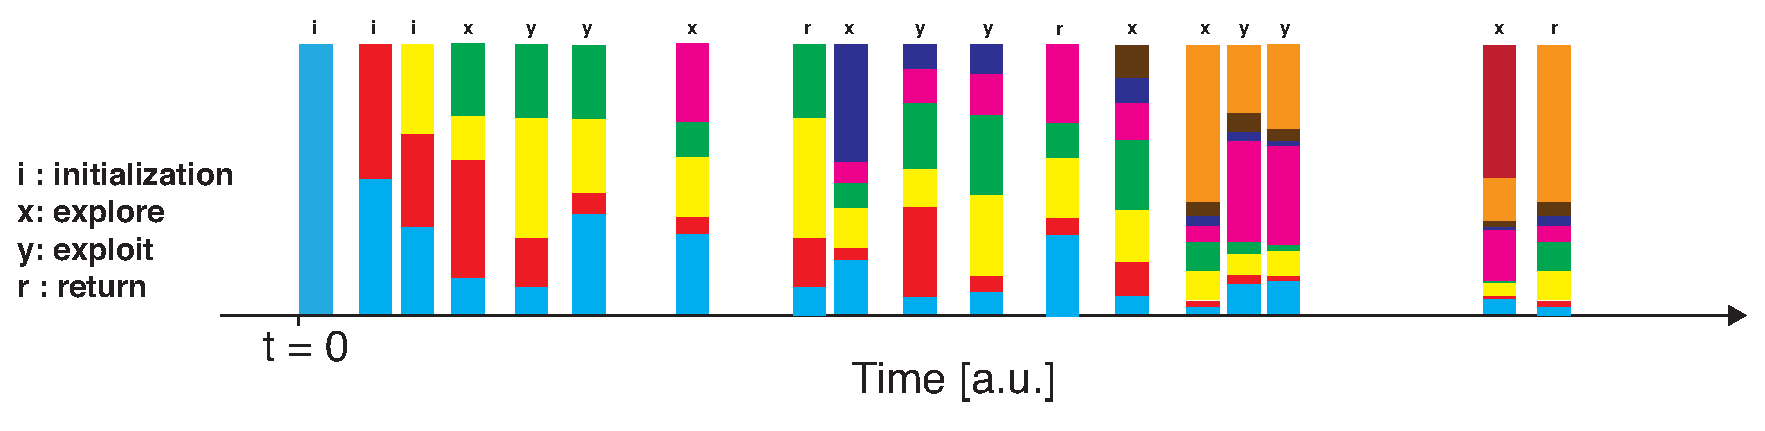
\includegraphics[width=16cm]{figures/schematic_remix.eps}
\caption{Schematic representation of remix dynamics. The color bars show the proportion (i.e., $1/d$) of previously proposed solutions in solution proposed at time $t$. New colors are introduced 	to signal exploration. From time to time, individuals return to previously visited solutions (signaled by $r$).}
\label{fig:schematic_remix}
\end{center}
\end{figure}


\begin{figure}[h!]
\begin{center}
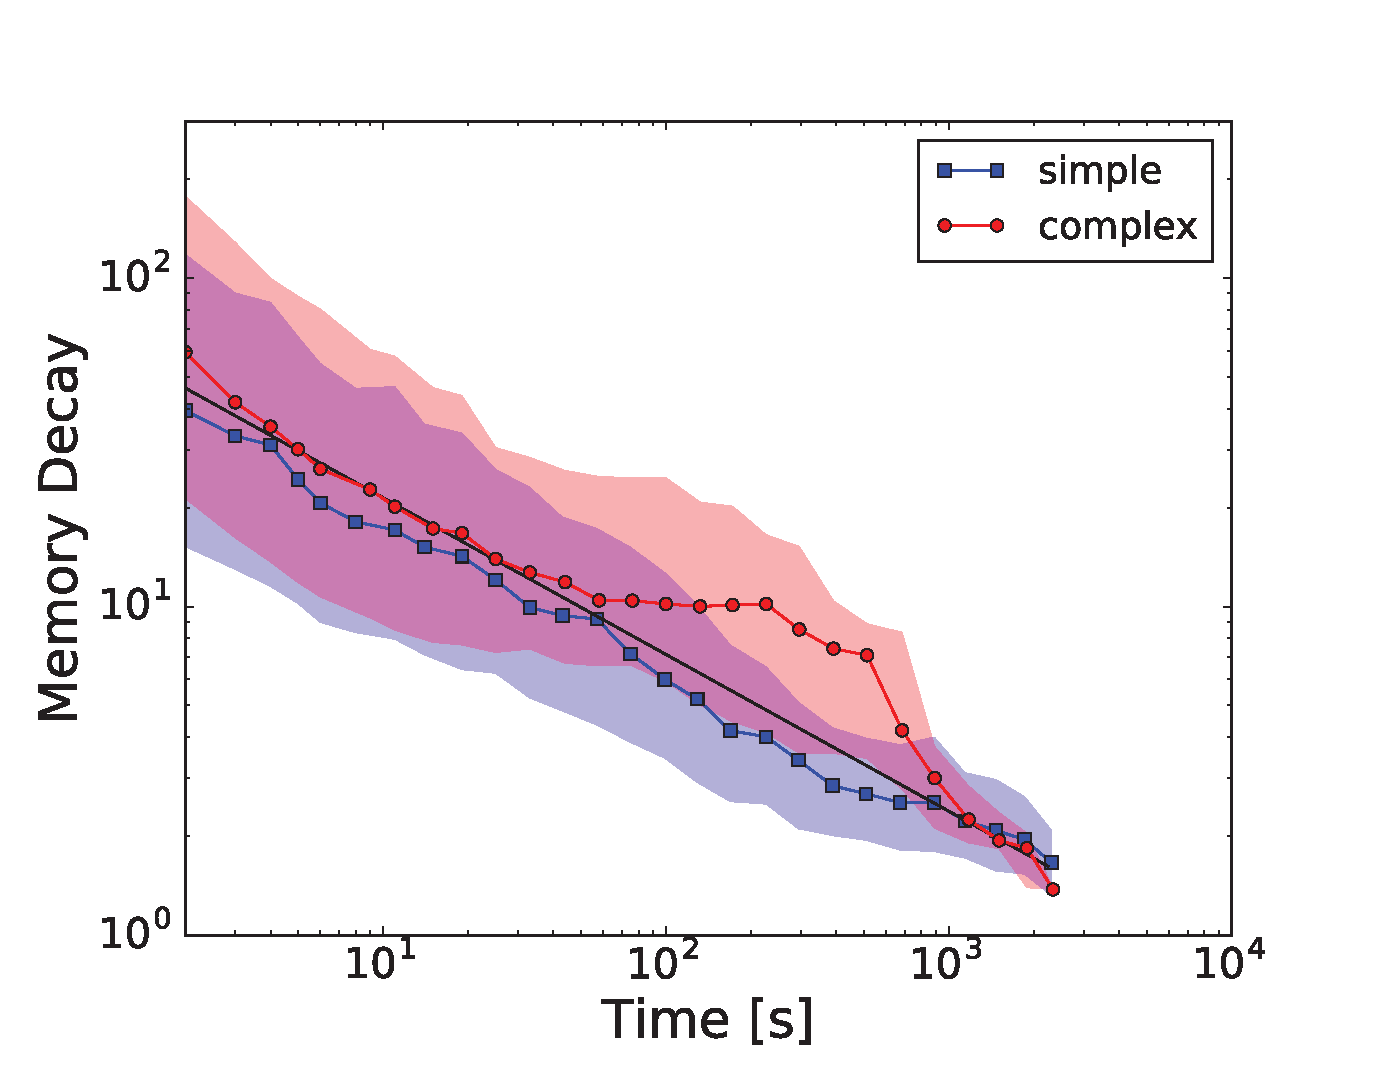
\includegraphics[width=13cm]{figures/MemoryDecay.eps}
\caption{Influence of a model proposed at time in subsequent models. The influence is computed as 1/distance between the focal model and subsequent models. On average over all participants in each treatment, influence $I$ decays as $I \sim t^{-\chi}$ with $\chi = 0.48(2)$ ($p < 0.01$ and $R > 0.32$). This result shows that memory is a long memory process, with implications for the convergence to.}
\label{fig:memory}
\end{center}
\end{figure}



%
%\begin{figure}[h!]
%\begin{center}
%\includegraphics[width=15cm]{figures/matrice2.png}
%\caption{\footnotesize The triangular matrix {\bf A} depicts the cognitive distances between a person's model at time $i$ and that same person's model at time $j$.  latest solution as a function of time and all former solutions, and {\bf B} of mean distance between the true model and resp. $i$ and $j$ configurations. Matrix {\bf B} shows the performance of a proposed model and serves as a reference for rationalizing choice sequences made by participants. These choice sequences are represented in matrix {\bf A} for participant 13: We see a wealth of characteristic choices leading to better of worse solutions, but also some integration and disruptive change in strategies, some which having a positive impact on performance, and other having a negative impact on performance. The rectangle structures show that participants do not drastically update drastically, but rather alternate periods of fine tuning and radical innovation. Matrix {\bf A} can also be watched in a more heuristic way at the coarse grained level: The more contrasted the pattern the more innovation overall. And, as shown here for participant 13, as more models are tested -- towards the lower right corner -- colors get more yellowish showing overall convergence of models. In the case presented here, the convergence of models leads overall to better solutions over time. It may not always be the case.}
%\label{fig:matrices}
%\end{center}
%\end{figure}






\clearpage
%




%\renewcommand\thesection{\Alph{section}}
\renewcommand\thesection{S\arabic{section}}
\setcounter{section}{0}

\renewcommand\theequation{S\arabic{equation}}
\setcounter{equation}{0}


\begin{center}
{\Large Supplementary Information}
\vspace{3cm}
\end{center}





\section{Literature Review}
The cognitive science and economics literatures have found much evidence in support of consistency with as well as deviance from human learning with Bayesian constructs of learning. On average, especially when incentives are high and tasks extremely simple, subjects update their beliefs based on new data in a way that is consistent with Bayes rule. However, at the individual level, there are large variations, as well as systematic departures under certain conditions.  In these literatures, comparing human learning to Bayesian updating, observed deviations can be organized in terms of "biases" or "heuristics".  Deterministic bias may have the consequence of underweighting or overweighting evidence ('law of small numbers' ) relative to base rates.  Such biases are in turn explained by the concept of availability heuristic (Griffin and Tversky 1992), which reduces data to examples that immediately come to mind, rather than by considering the exhaustive data of all previous experience and it has the consequence of slowing learning.  An example of the latter is recency bias \citep{FudenbergPeysakhovich2014}.  Another obstacle to efficient learning is when ambiguous information is taken to be a confirmation of a currently held hypothesis, or when information is suboptimally acquired or remembered.  Additionally, people have been found having difficulties with contingent reasoning with regards to future events \citep{CharnessLevin2009}. 
 
A different literature, associated with many disparate disciplines, such as ecology, cognitive science and complex systems frames learning and behavior in uncertain environments in terms of search, a ubiquitous property of life (Hills, Thomas T. et al. 2015).  Search, in turn, is a process of exploration and exploitation.  If behavior remains stable over some period of time, is focused and stays within a narrow subspace of the feasible decision or belief space it is interpreted as exploitation.  If it is erratic and moves wildly, it is interpreted as exploration (Mehlhorn et al, 2015).   

%These departures are clues to the heuristics humans use in their judgments, which overall often approximate bayesian inference but are not equivalent. Although many of these deviations imply that learning should be slower than predicted by Bayes rule,  few experiments measure the rate of learning and how far it departs from Bayesian inference.  

But why should one search and not simply count past events as Bayesian and Frequentist rationality demand (co-occurrences of values of a set of variables)?  With regards to counting observed frequencies of co-occurrences in order to measure covariances between a set of variables, if the number of variables gets large, the number of possible co-occurrences becomes astronomical.  Thus, remembering how many times a particular constellation of values of a given set of variables co-occurred puts ever increasing demands on memory as the set of variables gets large.  "In any system responsible for managing a vast data base there must be failures of retrieval" (Anderson, J. R., & Schooler, L. J. 1991).  Hence optimality must not mean Bayesian or Frequentist optimality, as counting all possible co-occurrences is not feasible because of limits on memory.  Additionally, there is the problem of assigning beliefs to never before experienced co-occurrences.  Note that Anderson, J. R., & Schooler, L. J. 1991 present not an argument about specific human biases or heuristics but rather one that presupposes a different definition of optimality that takes natural limits into consideration.  Our work begins with this same definitional premiss.  In addition to their own findings, Anderson, J. R., & Schooler, L. J. 1991 review the pervasive findings of power functions in the learning literature with respect to positive and negative performance measures and time.  As long as the performance measure is either unbounded or does not approach its bounds, the relationship between performance and time seems to follow the functional form:
$$P = A*T^{b},$$
where $b$ is negative and $P$ can either have negative valence, such as number of trials necessary to learn someone's name, or positive valence such as probability of having retained a name. In our case, the measure is bounded, above by 1 and below by 0, but never approaches either of its bounds. 

Learning of statistical systems can also be seen as search processes in simplex-spaces. If we consider learning as searching with feedback and we may do so if we find that brains learn as brains search, then another literature becoomes relevant that has not been generally considered by those studying learning; the literature concerened with foraging and the sort of spacial learning that had been most relevant throughout human evolution.  For most of our evolutionary history there were no stock and insurance markets and thus there is no reason to believe that our brains were optimized for the sort of learning that is optimal in those modern scenarios.      
%We find that it is not (slower). Furthermore, we also find that the quality of the inferences at each time space and across players varies a lot, following a "punctuated equilibrium" pattern. These observations are thus additional clues about the cognitive processes at play, with fine-grained information about how subjects update their beliefs in response to new information and the success and failure of their bets. Below were review some of the promising cognitive mechanisms posited to explain some of the deviations above and which can be evaluated in light of our data.

%2) Cognitive mechanisms 
%Interesting mechanisms have to do with how people organize the hypothesis space and sample from it. 
%- sampling hypothesis
%- change of paradigm when observing "surprising events" (Ortoleva)

%the satisficing principle may also mediate the learning process because computations such as bayes rules are costly. 

\section{Problem Formulation}
\subsection{Intuition}

Random search processes occur in many areas, from the foraging behavior
of bacteria and animals \cite{}, to human mobility \cite{}, to computer search and optimization algorithms \cite{}.  When searching for solutions to outstanding problems, humans must come up with innovative solutions, which involve random search (e.g., gathering information, etc), along with the consolidation of past and current experience.

Here, we show how people go through the resolution of a complicated problem, starting from no knowledge through L'evy random search, involving synthesizing current knowledge versus exploring out-of-the box (see Figure \ref{fig:schematic}). We then measure how this process leads to convergence, albeit very slow convergence, to the solution.

%{\bf huge mistake?:  the displacement is not necessarily the path to a better solution. JS-Distance is a by-product of displacement (of the search process) $\rightarrow$ JSD is the objective function NOT the process}

\subsection{Simple case}

The intuition is that large jumps lead to super-diffusion while long-waiting time lead to sub-diffusion. Here, we see both large jumps and long waiting time. There is thus a tension between the two factors and how they respectively influence the random search process. However, both are correlated: larger waiting times lead to larger jumps, yet with a decreasing marginal function ($\Delta r \sim {(\Delta t)}^{\nu},~with ~\nu \approx 0.23 < 1$). This suggests that waiting time may trigger more aging (sub-diffusion), compared to long-range search (i.e., super-diffusion), which has been found to be an optimal search \cite{optimal_random_search}. In turn, the




\subsubsection{Jump size}

\be
P(\Delta r) \sim r^{-(1+\alpha)},~with~\alpha = 0.61(3).
\ee

with upper cut-off $max(\Delta r) \approx 1$ close to the absolute max ($2\sqrt{2} \approx 2.83$).

\subsubsection{waiting times}

\be
P(\Delta t) \sim t^{-(1+\beta)},~with~\beta = 0.46(3).
\ee

with a change of regime for $\Delta t > 100$ (in that case: $\beta = 1.65(1)$).

\subsubsection{dependence between $\Delta r$ and $\Delta t$}

nb: We find a dependence (Spearman rank correlation $corr = 0.32$) between  $\Delta r$ and $\Delta t$, which can be approximated by

\be
\Delta r \sim {(\Delta t)}^{\nu},~with ~\nu = 0.23(2)
\ee


\subsubsection{mean square displacement}

\be
MSD = \langle r(t)^2 \rangle = t^{\gamma},~with~\gamma = 0.35(1).
\ee

$\rightarrow$ subdiffusion

\subsubsection{Number of distinct locations visited}

\be
S(t) \sim t^{\mu},~with~\mu = 0.85(0)
\ee

\begin{center}
\ba
\Delta S / \langle S \rangle = S^{0.33(2)}\\
%\ee
~or~\\
%\be
\Delta S / \langle S \rangle = e^{-\lambda S},~with~\lambda = 1.6\times 10^{-2}
\ea
\end{center}



\clearpage



\subsection{Jensen-Shannon Distance}


\begin{equation}
{\rm JSD}(P \parallel Q)= \sqrt{\frac{1}{2}D(P \parallel M)+\frac{1}{2}D(Q \parallel M)}
\end{equation}
where $M=\frac{1}{2}(P+Q)$


The Jensen-Shannon Distance (JSD) is a measure of mutual information. We use it to compare the distance of a BayesNet model from the true model (see Figure \ref{fig:decay}), and between models.\\


Score:
\begin{equation}
S = 1 - JSD
\end{equation}



\subsection{Ultra Slow Diffusion / Power Law Decay}

The CTRW model predicts that the mean square displacement (MSD) asymptotically follows $\langle \Delta x^2 (t) \rangle \sim t^{\nu}$ with $\nu = 2\beta /\alpha$

\begin{equation}
\label{power_law_decay}
JSD(t) = C \cdot t^{-\alpha},
\end{equation}

with $\alpha = 0.09$ and $C$ a constant, specific to the $simple$ and $complex$ models

\begin{equation}
\label{ultraslowdiffusion}
S(t) = 1 - JSD(t) = 1- C \cdot t^{-\alpha},
\end{equation}


\subsubsection{Stepwise Jumps}

\begin{equation}
P(R > \Delta r) \sim |\Delta r|^{-\alpha}, ~~with~~\alpha \approx 0.1,
\end{equation}

jump size $\Delta r$ Figure \ref{fig:jump_sizes}



\subsubsection{Memory Effects / Waiting Times}

waiting time $\Delta t$


Figure \ref{fig:waiting_times}

\begin{equation}
P(T > \Delta t) \sim |\Delta t|^{-\beta}, ~~ with~~  1< \beta < 2
\end{equation}



\subsubsection{Continuous Time Random Walk (CTRW)}

continuous-time random walk (CTRW)  $\rightarrow$ is a generalization of a random walk where the wandering particle waits for a random time between jumps. It is a stochastic jump process with arbitrary distributions of jump lengths and waiting times.[1][2][3] More generally it can be seen to be a special case of a Markov renewal process.

\begin{equation}
\psi(\Delta r,\Delta t)=P(\Delta r)P(\Delta t)
\end{equation}

with $P(\Delta r)$ and $P(\Delta t)$ are not dependent.

{\bf Jump length pdf :}
\begin{equation}
\lambda(\Delta r) = \int_0^{\infty} dt \psi(\Delta r,\Delta t)
\end{equation}

{\bf Waiting Time pdf :}
\begin{equation}
w(\Delta t) = \int_{-\infty}^{\infty} dx \psi(\Delta r,\Delta t)
\end{equation}

Characteristic waiting time:
\begin{equation}
T \int_0^{\infty} dt w(t)t
\end{equation}


Characteristic waiting time:
\begin{equation}
\Sigma^2 = \int_{-\infty}^{\infty} dx \lambda(x) x^2
\end{equation}


\subsection{Number of distinct locations / Visitation frequency:}

(A) The number of distinct locations $S(t)$ visited by a randomly
moving object is expected to follow:


\begin{equation}
S(t) \sim t^{\mu}
\end{equation}


where $\mu = 1$ for LŽvy flights [24] and $\mu = \beta$ for CTRW. {\bf [Here, it is unclear what visiting a distinct location means ]}
The probability $f$ of a user to visit a given location is expected to be asymptotically uniforma ($f\sim const.$) for both LŽvy flights and CTRWs. In contrast, the visitation patterns of humans is rather uneven, so that the frequency $f$ of the $k$th  most visited location follows

\begin{equation}
f_k ~k^{-\zeta}
\end{equation}

where $\zeta \approx 1.2 \pm 0.1$ (babarasi paper).


\subsection{slight anisotropy}
The propagator is anisotropic: There is equal chance that a jump will be negative or positive. However, the distribution of jump size is different: both are power law, but with different exponents.

isotropy :
\begin{equation}
W_j (t+\Delta t) = a W_{j-1}(t) + b W_{j+1}(t)
\end{equation}

with $a=b=1/2$. In case of anisotropy $\rightarrow  a \neq b$.



\subsection{Exploration versus Exploitation}
Each new BayesNet iteration may be a combination of former iterations, or rather something new. It is difficult to determine if {\it exploration} occurs, by opposition to {\it exploitation}. The intuition is that if the sum of distances between the new node and all existing nodes (weighted by their iteration number) is larger than at the previous step, then more exploration occurs

\begin{equation}
\overline{JSD}(N) =  \sum_{n=0}^{N-1} \frac{JSD(n,N)}{n}
\end{equation}



\subsection{Formulation of reuse, with memory}

\section{Measures of Cognitive Distance}

In this section, we will introduce various measures.  We use the square root of a measure called the Jensen Shannon Divergence as our measure of cognitive distance (CD). The performance score is then

\begin{equation}
S = 1 - CD.
\end{equation}

In order to understand the usefulness and reason behind this measure this section introduces some preliminary measures which the Jensen-Shannon Divergence builds on and then formally defines our measure of cognitive distance.    
  
\subsection{The Shannon Entropy}

An important measure of ignorance is the Shannon Entropy, which is maximized whenever all possible events are believed to occur with equal probability:

$H(X)=-\sum_ip_i(x_i)\log(p_i(x_i)).$

The entropy of a stochasic process, $\{X_i\}$ is defined by 

$H(\chi)=\lim_{n\rightarrow\inf}\frac{1}{n}H(X_1, \ldots, X_n),$

when the limit exists, which in this case it does as it was picked by us. 
We can calculate, then, that the Shannon Entropy of the simple ``treatment'' system is $2.7$ and that of the complex one is $3.26$. However, distributions over larger alphabets tend to have higher entropy and for our purposes the entropy should be considered a relative measure over distributions of the same cardinality. 

Specifically, the maximum entropy for categorical variables with $N$ categories is $\log_2(N)$, which happens when for each category, $x_i$, its probability is $p_i(x_i)=\frac{1}{N}$. 

This fact can be appreciated on hand of a mental or computational experiment \citep{Cover13} where there is an automatic type writer that randomly prints a sequence of letters from an alphabet with $m$ members, where at each time, $t$, each member of the alphabet has an equal chance of $\frac{1}{m}$ to be chosen as the next member of the sequence. The type writer can produce $m^t$ possible sequences of length $t$, each of them as likely as any other. We then have that 

$H(X_1, \ldots, X_t)=\log(m^n)$ and the entropy rate is $H(\chi)=\log m$ bits per symbol. 

In the current case, we can substitute $m$ with the number of possible combinations (joint states) that $k$ binary variables can assume: $2^k$.
The simple system has $k=3$ binary variables and its maximum entropy (random type writer) belief has entropy $\log_2(N)=\log_2(2^k) = 3$. The more complex treatment system has $k=4$ binary variables and thus its maximum entropy belief has entropy $\log_2(N) = 4$. Entropy is also always positive, so that the measure is bounded between $0$ and the logarithm of the number of joint states $2^k$ that define the system. The Shannon Entropy is measured in bits when the base $2$ logarithm is used and it can be interpreted as the average number of yes or no questions a person needs to ask someone who knows the current outcome in order to gain knowledge of it.  In the worst case, this requires as many yes or no (high, or low) questions as there are binary variables, $k$. 

\begin{figure}
\noindent\makebox[\textwidth]{%      
        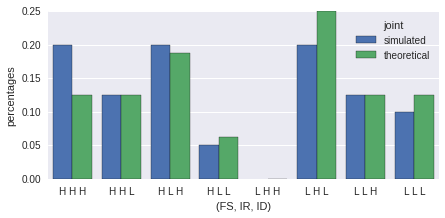
\includegraphics[width=1\textwidth]{figures/simplejoint.png}}
\caption{The limiting distribution of the simple treatment and an example frequency distribution pertaining to 400 random realizations.}
\label{fig:simplejoint} 
\end{figure}

But it is easy to see from a picture of the joint distribution describing joint behavior of the simple system (Figure \ref{fig:simplejoint}), for example, that very often three questions won't be needed. We could ask the person who knows whether the first variable, labeled ``Financial Sector'', has taken on the value ``H''.  If the answer is no, we could ask if the outcome is the event ``L'', ``H'', ``L'' and very often we would be right, finding the answer with only $2$ yes or no questions. Better yet, if we knew or somehow guessed the correct causal structure, we would know that whenever the ``Financial Sector'' variable takes on the value ``L'' and the ``Interest Rate'' variable assumes the value ``H'', the ``Industry'' variable must be in the low state. So, if we asked first ``is the value of the Financial Sector high'' and received ``no'' as an answer and then we asked ``is the value of the Interest Rate high'' and we received ``yes'' as an answer, we could be certain that the outcome must be ``LHL''. On average, for the simple system we would need to ask $2.7$ yes or no questions, if we know the distribution.   

\subsection{The Kullback-Leibler divergence}

The Kullback-Leiber Divergence was proposed as a measure of difference between two probability distributions $P$ and $Q$. Specifically, it was meant as a measure of the information that is lost when belief $Q$ is used as an approximation for a true probability distribution $P$:
\\

$D_{KL}(P(X) | | Q(X))=\sum_ip_i\log_2(\frac{p_i}{q_i}).$
\\

It is readily apparent that the Kullback-Leibler divergence can be re-expressed as follows:
\\

$D_{KL}(P(X) | | Q(X))=\sum_i (p_i\log_2p_i -p_i\log_2q_i = H(P, Q)-H(P)$, 
\\

where $H(P, Q)$ is known as the cross-entropy of $P$ and $Q$, and $H(P)$ is simply the entropy of $P$.

There are two problems with the Kullback-Leibler divergence as a measure of distance: 1) it is not symmetric ($D_{KL}(P | | Q) \not= D_{KL}(Q | | P)$) and 2) for the two distributions $P$ and $Q$, if one of the $q_i$ is equal to $0$, but the corresponding $p_i$ is not equal to $0$, the measure is not defined.  For example, we can see that when we simulated the complex process, some of the theoretically rare but possible outcomes have not yet occurred during the simulation and thus, if we want to measure the distance between the theoretical distribution and the frequencies of the simulated outcomes, using the Kullback-Leibler divergence, we will find that this measure is not defined. 

\subsection{The Jensen–Shannon divergence}

The Jensen–Shannon divergence is a symmetrized version of the Kullback-Leibler divergence that also solves the zero division problem:
\\

$D_{JS}(P | | Q)=\lambda*D_{KL}(P | | M) + (1-\lambda)*D_{KL}(Q | |M),$ 
\\

where $M=\lambda P + (1-\lambda) Q$ and $\lambda$ is usually, but not necessarily equal to $\frac{1}{2}$. In order for the measure to be symmetric, $\lambda$ has to be equal to $\frac{1}{2}$. 


The value of the Jensen-Shannon divergence is always between $0$ and $1$; $0$, when the two distributions are the same and $1$ when the two distributions have orthogonal support. This measure quantifies the amount of information in bits, about which of the two distributions one bit of data was drawn from, given that it was drawn from the first distribution with probability $\lambda$ and from the second with probability $1-\lambda$. For example, if the two distributions are the same, any bit of data will render no information about which of the two identical distributions it was drawn from, while if the two distributions have orthogonal support, each bit of data gives exactly one bit of information. To state this in Bayesian terms: if the two distributions are the same, then we can not learn from data and our posterior probability about which of the two distribution that data was drawn from is equal to our prior ($\lambda$ for the first distribution). At the other extreme, if the distributions have orthogonal support, the posterior will put probability $1$ on the distribution that supports the data; one bit of data carries one bit of information. 

\subsection{Cognitive Distance and the Performance Score}

If the square-root of the Jensen-Shannon divergence is taken, the result is a metric known as the Jensen-Shannon distance. This is the distance metric we use to calculate distances between any two distributions.  We refer to it as Cognitive Distance (CD):

\begin{equation}
CD(P, Q) = \sqrt{D_{JS}(P | | Q)}
\end{equation}

and to remind the reader, our performance score of person $i$ at time $t$, (supressing the index $i$), $S_t$, is 

\begin{equation}
S_t = 1 - CD(M_t, T),
\end{equation}

where $M_t$ is some person's Bayes Net model, at time $t$, of the true stochastic system, $T$. 



\end{document}




 


